\documentclass{beamer}	
\mode<presentation>
 
\usepackage{pdfpages}
\usepackage{fancyvrb}
\usepackage{chemarr}

\usepackage{amsmath}		%% mathematics typesetting
\usepackage{amssymb}
 
\usepackage{epigraph}   %% nice setting of quotations

\usepackage{tabularx} %% allows to use row colours in tables

\usepackage{ulem}

\usepackage{booktabs}

\usepackage{siunitx} %% tpyeset SI units

\usepackage{CJKutf8} %% typeset Chinese characters

\usepackage{pdfpages}%% include pdfs


\usepackage{animate} %% show animated gifs

\DeclareMathAlphabet{\mathcalligra}{T1}{calligra}{m}{n}


% Color and Theme. Can be changed. However, this one's quite nice.
\usetheme{Madrid}
\definecolor{theme}{rgb}{0.84,0,0.21}
\usecolortheme[named=theme]{structure}


%%  Title information
\title[M01.5 Schwingungen und Wellen]{M01.5 Schwingungen und Wellen}
\author[melanie.stefan@medicalschool-berlin.de]{M01 Physik für Mediziner*innen}
\institute[]{Prof. Melanie Stefan - melanie.stefan@medcialschool-berlin.de}
\date{WiSe 2022/23}
 

% Table of contents to pop up at the beginning of each section
\AtBeginSection[]
{
  \begin{frame}<beamer>
    \frametitle{Outline}
    \tableofcontents[currentsection,currentsubsection]
  \end{frame}
}
 
\beamertemplatenavigationsymbolsempty

\begin{document}
 
  { \usebackgroundtemplate{
\includegraphics[width=1.2\paperwidth]{MSB_Titelseite.pdf}} 
\begin{frame}

 \maketitle 

$\,$\\[6cm] 


\end{frame} 
}


%% Hook: Evelyn Glennie

{
  \usebackgroundtemplate{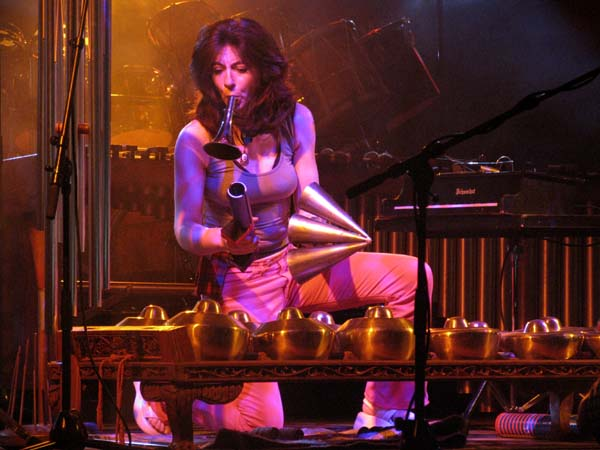
\includegraphics[width=1.2\paperwidth]{evelyn_glennie.jpg}}

\begin{frame}[plain]
% \frametitle{Evelyn Glennie}





\end{frame}
}


%% TLIA
{
  \usebackgroundtemplate{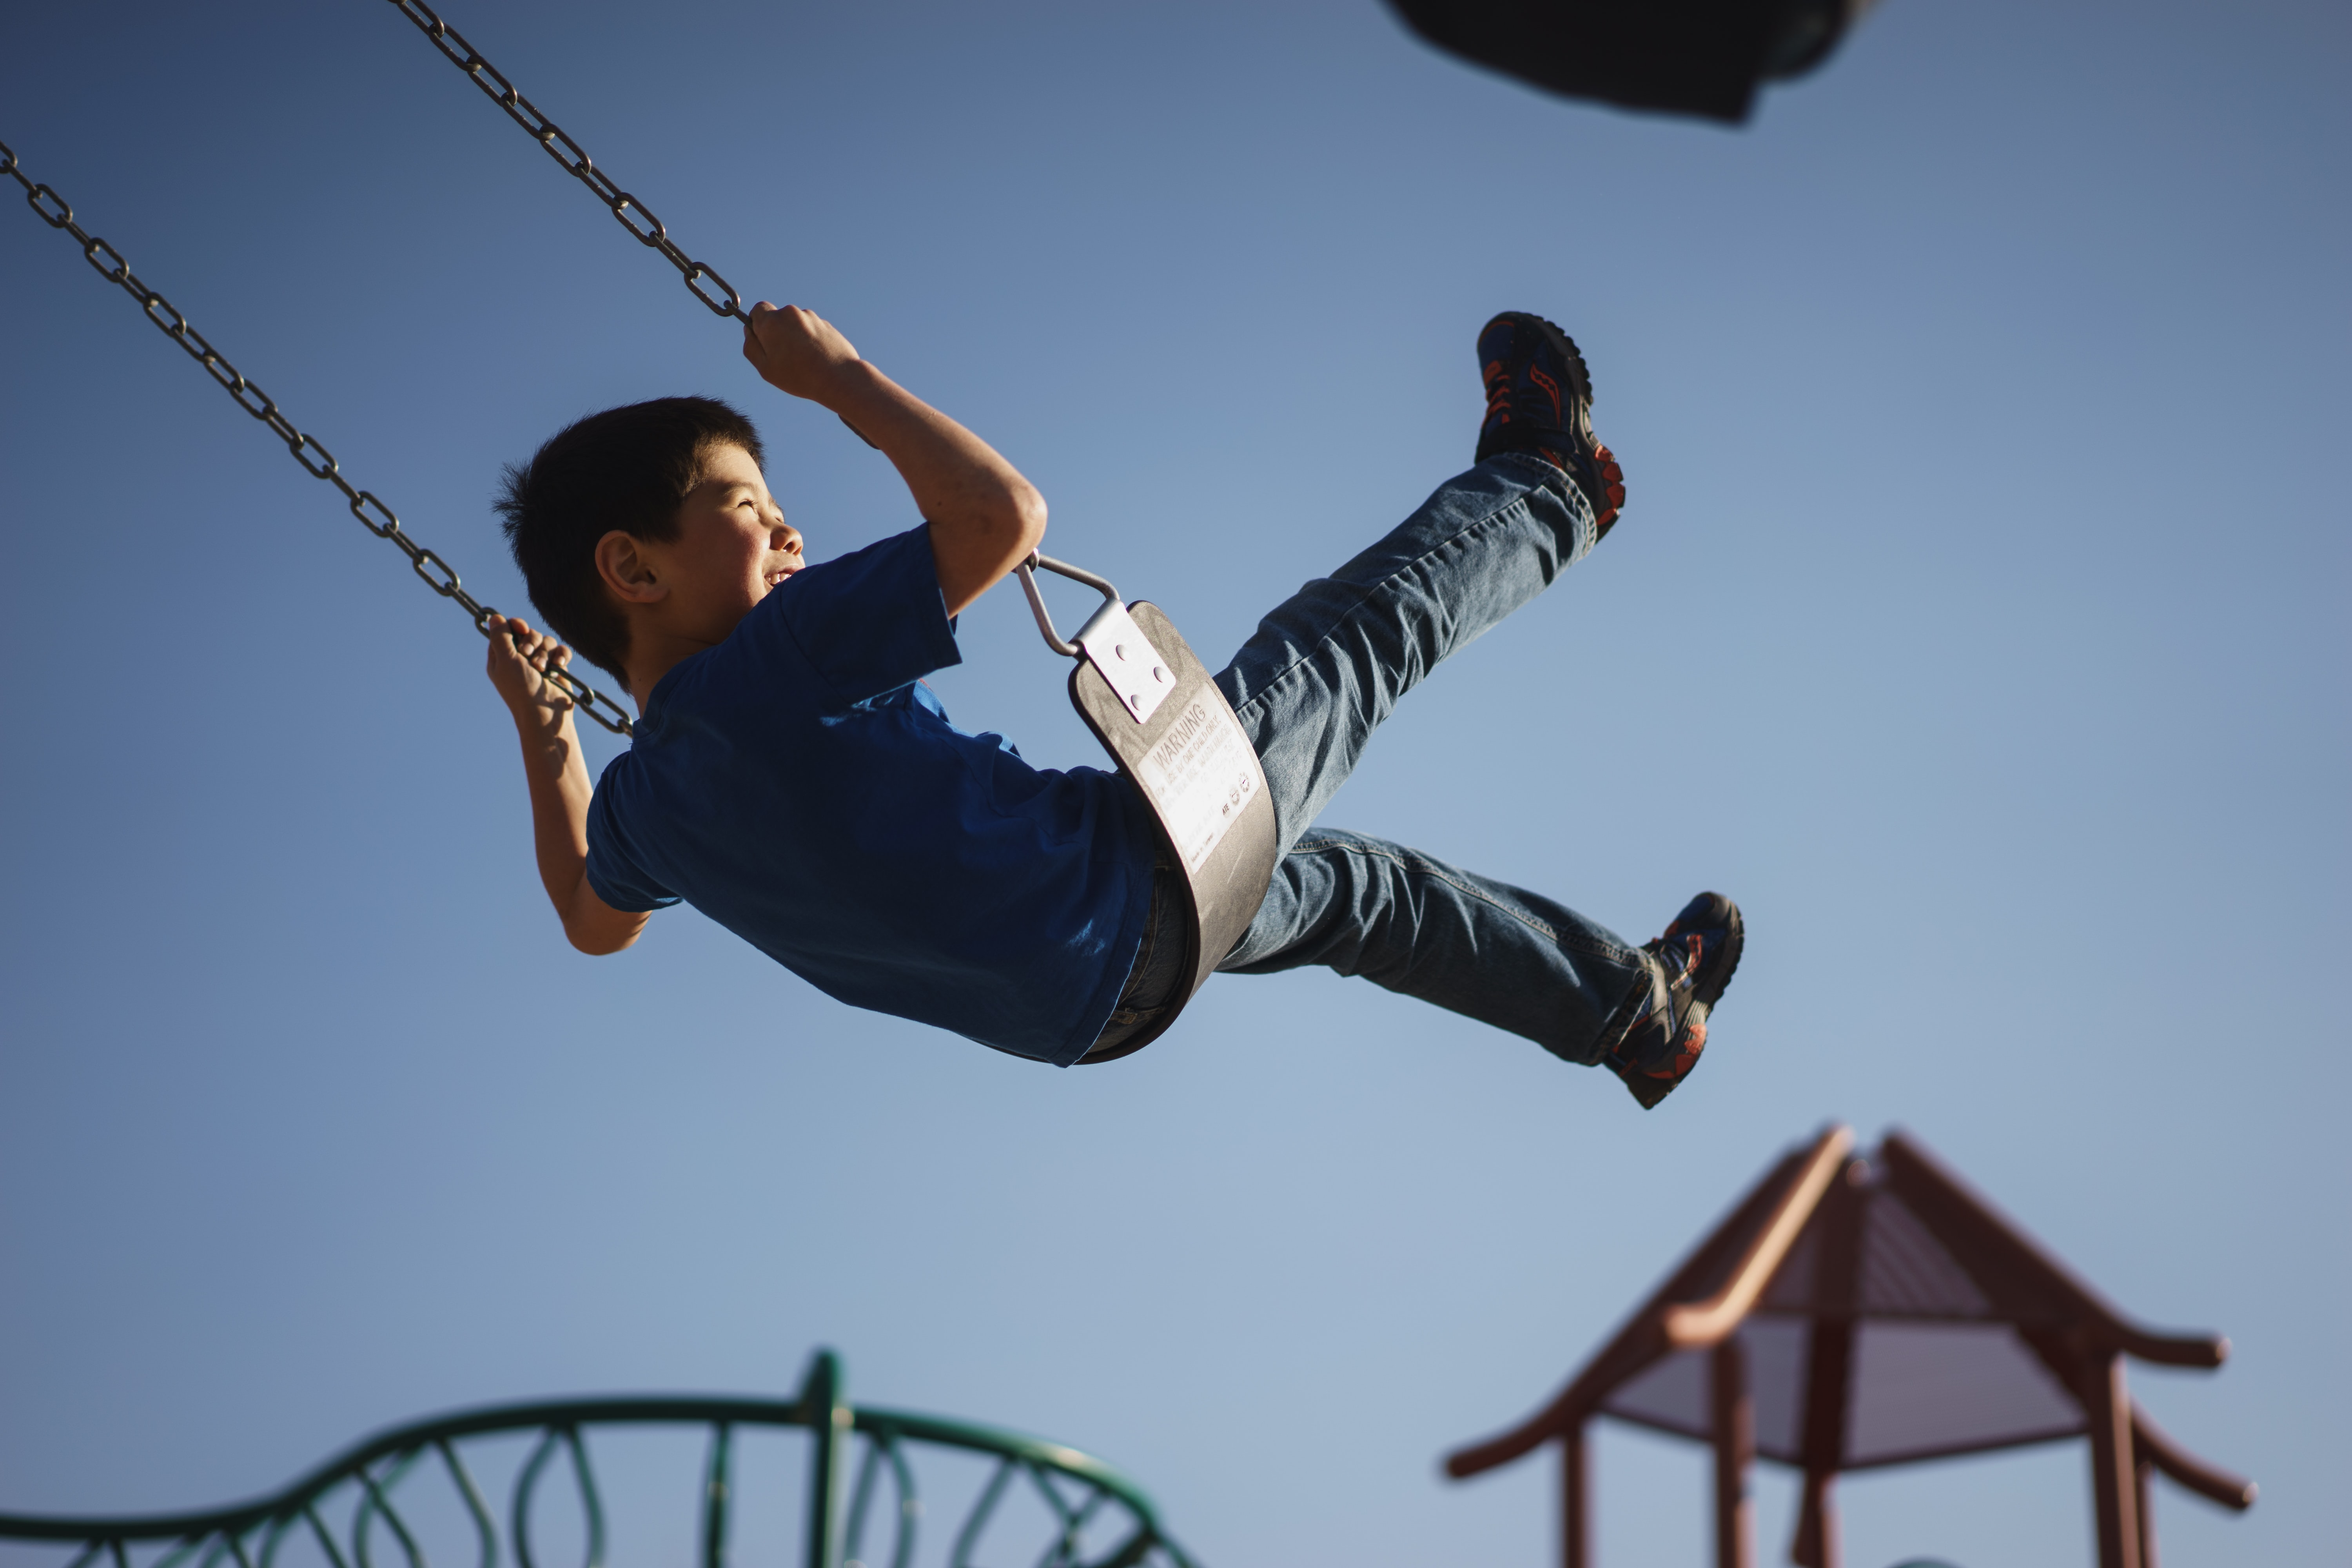
\includegraphics[width=1.2\paperwidth]{schaukel.jpg}}
  
\begin{frame}[plain]

\frametitle{In dieser Vorlesung geht es um \dots}

$\,$\\[5cm]


\Large{Schwingungen und Wellen}


 
\end{frame}
}




%% Learning Objectives
 
\begin{frame}

\frametitle{Nach dieser Vorlesung sollten Sie:}



\begin{block}{Wissen:}
\begin{itemize}
%%%%%
\item
Schwingungen und Wellen definieren
\item
Charakteristika von Schwingungen und Wellen benennen 
\item
Arten von Schwingungen und Wellen unterscheiden
\item
Erzwungene Schwingungen definieren und erklären
\item
Phänomene bei der Überlagerung von Wellen erklären
\item
Den Doppler-Effekt erklären
\item
Beispiele für den Doppler-Effekt geben
\item
Eigenschaften von Schallwellen benennen
\item
Eigenschaften elektromagnetischer Wellen benennen
\item
Unterschiede und Gemeinsamkeiten zwischen elektromagnetischen Wellen und Schallwellen angeben
\item
Das Konzept der Fourieranalyse erklären und Anwendungen nennen
\end{itemize}

\end{block}

\end{frame}

\begin{frame}

\frametitle{Nach dieser Vorlesung sollten Sie:}
 

\begin{block}{Können:}
\begin{itemize}
\item
Charakteristika von Schwingungen und Wellen berechnen
\item
Graphische Darstellungen von Schwingungen und Wellen interpretieren
\item
Änderungen der Schallstärke berechnen
\item
Mit Klavieren experimentieren (und auch sonst) 
\end{itemize}
\end{block}

\begin{block}{Fühlen:}

\begin{itemize}
\item
Keine Angst vor Fouriertransformationen haben
\item
Schwingungen und Wellen im Alltag sehen 


\end{itemize}

\end{block}


\end{frame}


%% Main Body


%%%%%%%%%%%%%%%%%%%%%%%%%%%%%%%%%%%
%% Schwingungen
%%%%%%%%%%%%%%%%%%%%%%%%%%%%%%%%%%%

\section{Schwingung}

%% Was sind Schwingungen
\begin{frame}
\frametitle{Schwingung (Oszillation)}

\begin{columns}[c]
\begin{column}{7cm}
Wiederholte zeitliche Veränderung in einem System \\[1 cm]

\pause

Beispiel: Fadenpendel

\end{column}
\pause
\begin{column}{3cm}


\begin{center}
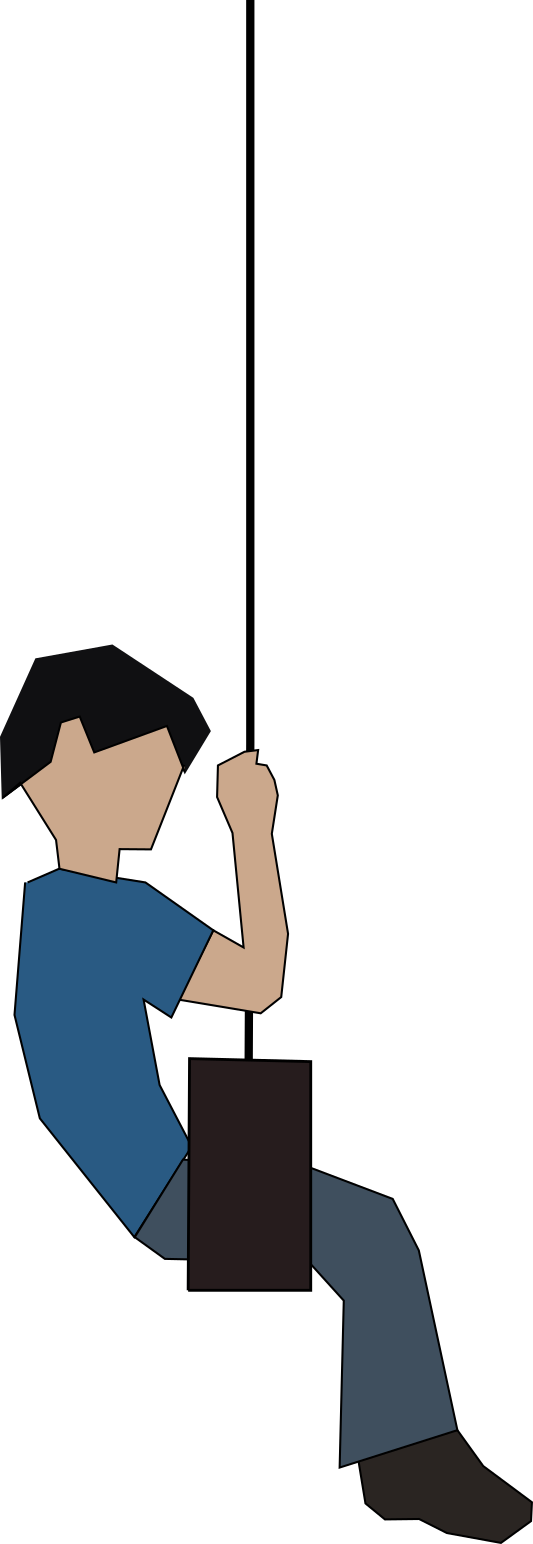
\includegraphics[width=0.5\textwidth]{/home/melanie/Work/pictures/physics/kind_schaukel.png}
\end{center}



\end{column}

\end{columns}



\end{frame}


%% Schwingungen zeichnen
\begin{frame}
\frametitle{Schwingungen können als Zeitreihe gezeichnet werden}

\begin{center}
\includegraphics<1>[width=0.2\textwidth]{/home/melanie/Work/pictures/physics/schaukel_sinus_1.png}
\includegraphics<2>[width=0.2\textwidth]{/home/melanie/Work/pictures/physics/schaukel_sinus_2.png}
\includegraphics<3>[width=0.2\textwidth]{/home/melanie/Work/pictures/physics/schaukel_sinus_3.png}
\includegraphics<4>[width=0.2\textwidth]{/home/melanie/Work/pictures/physics/schaukel_sinus_4.png}
\end{center}

\end{frame}


%% Schwingungen: Charakteristika
\begin{frame}
\frametitle{Schwingungen charakterisieren}


\begin{center}

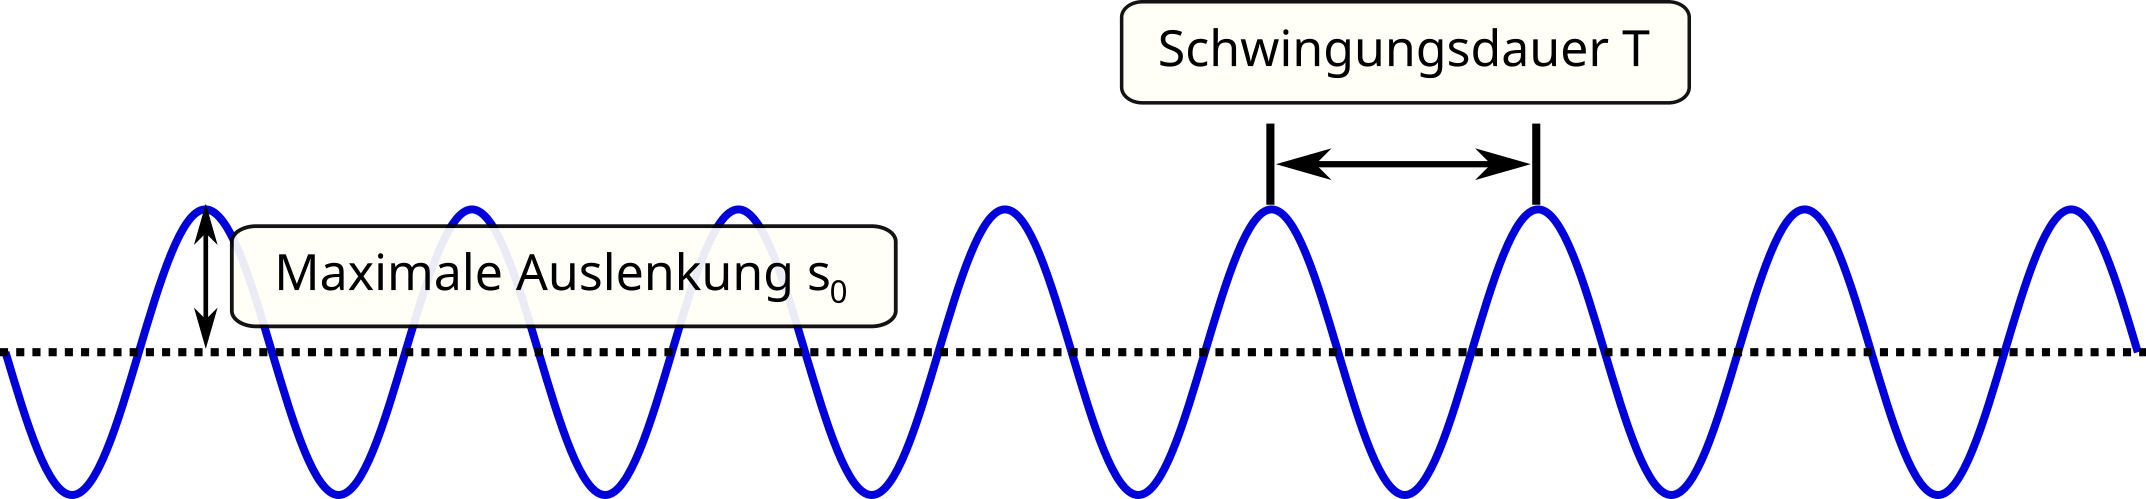
\includegraphics[width=\textwidth]{/home/melanie/Work/pictures/physics/schwingungen_groessen.png}
\end{center}

\pause

Auslenkung \(s\) zum Zeitpunkt \(t\)

\[
s(t) = s_0\sin\frac{2\pi t}{T} \pause =  s_0\sin 2\pi\nu t = s_0 \sin \omega t
\]

(bei Frequenz \(\nu = \frac{1}{T}\) und Kreisfrequenz \(\omega = 2\pi\nu\))

\end{frame}

%% Gedämpfte Schwingungen
\begin{frame}
\makebox[\linewidth]{\includegraphics[page=7,width=\textwidth]{Walter_Wellen.pdf}}
\end{frame}



%% Erzwungene Schwingungen: Central pattern generator

\begin{frame}
\frametitle{Erzwungene Schwingungen}

\begin{columns}[c]

\begin{column}{3cm}

\begin{center}
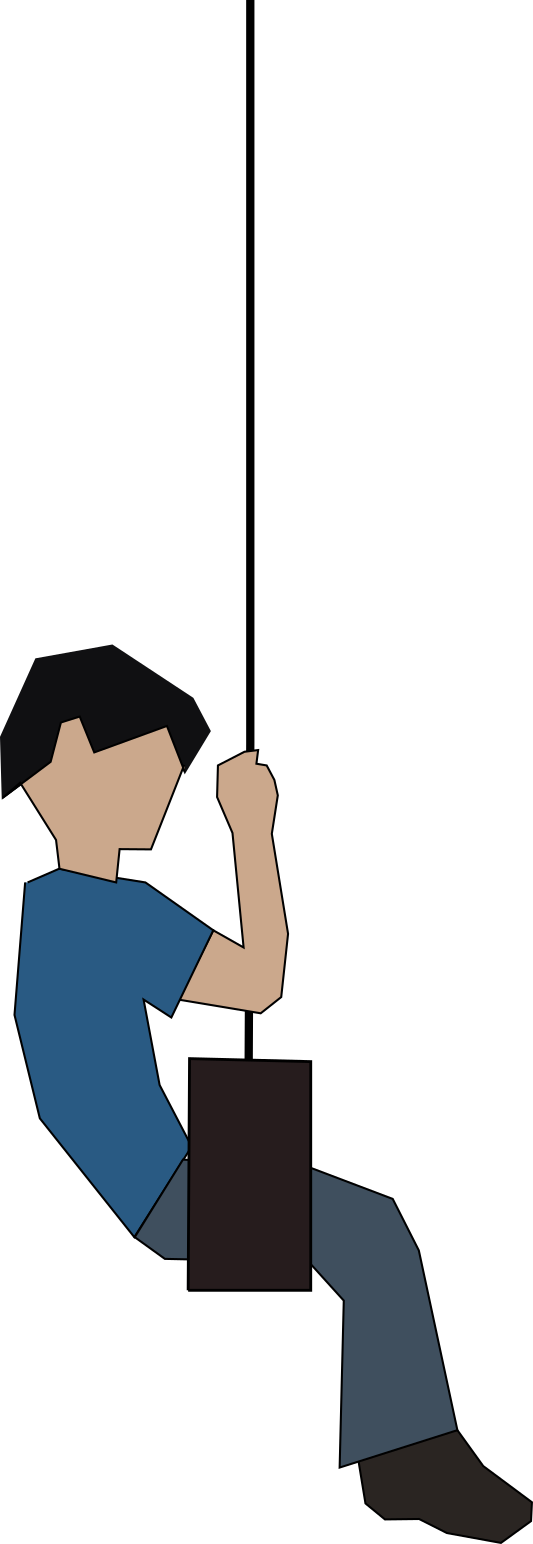
\includegraphics[width=0.5\textwidth]{/home/melanie/Work/pictures/physics/kind_schaukel.png}
\end{center}

\end{column}

\begin{column}{7cm}

\begin{itemize}
\item
Kind schaukelt mit Frequenz \(\nu_1\)
\item
Jemand  taucht an mit Frequenz \(\nu_2\)
\item
Was passiert?
\end{itemize}

\end{column}

\end{columns}
\end{frame}


\begin{frame}
\frametitle{Erzwungene Schwingungen}

\begin{columns}[c]

\begin{column}{3cm}

\begin{center}
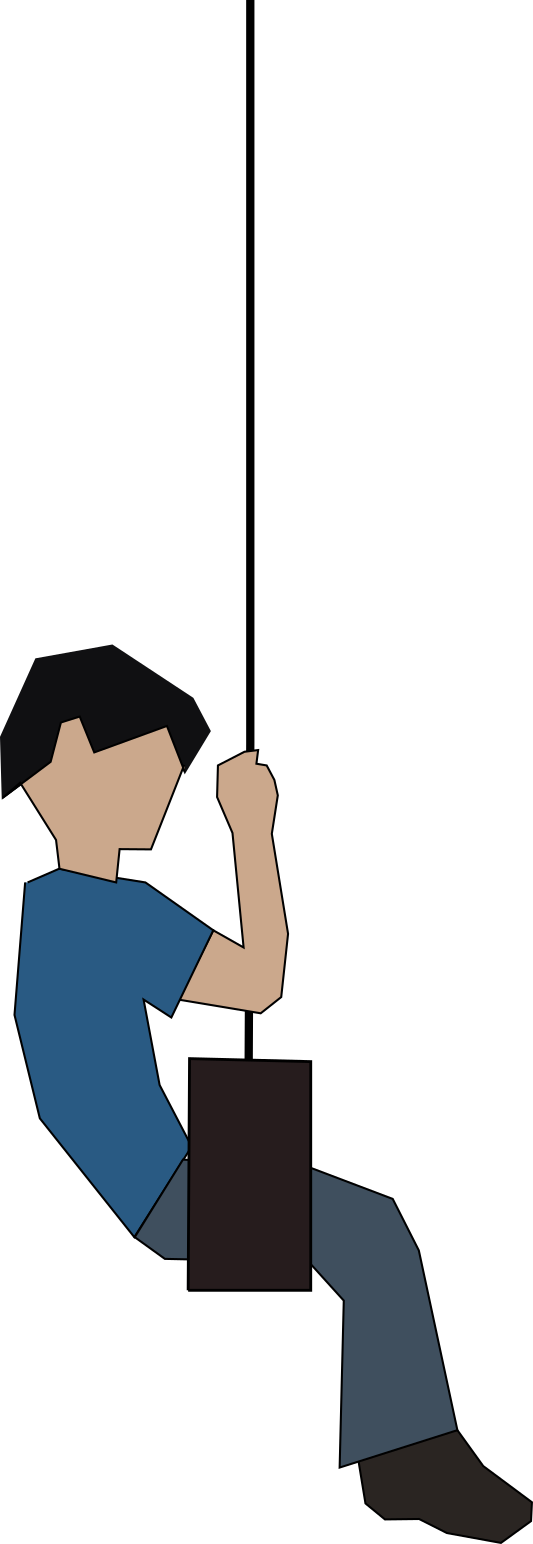
\includegraphics[width=0.5\textwidth]{/home/melanie/Work/pictures/physics/kind_schaukel.png}
\end{center}

\end{column}

\begin{column}{7cm}

\(\nu_1\), \(\nu_2\) sehr verschieden: Frequenz der Schaukel passt sich der Frequenz der antauchenden Person an. \\

\pause

\begin{block}{Beispiel: Central Pattern Generator}

Systeme von oszillierenden Neuronen, die einander beeinflussen und dadurch mit gleicher Frequenz schwingen. Verantwortlich für rhythmische Abläufe, z.B. Koordination der linken und rechten Körperhälfte beim Gehen.

\end{block}


\end{column}

\end{columns}
\end{frame}



\begin{frame}
\frametitle{Erzwungene Schwingungen}

\begin{columns}[c]

\begin{column}{3cm}

\begin{center}
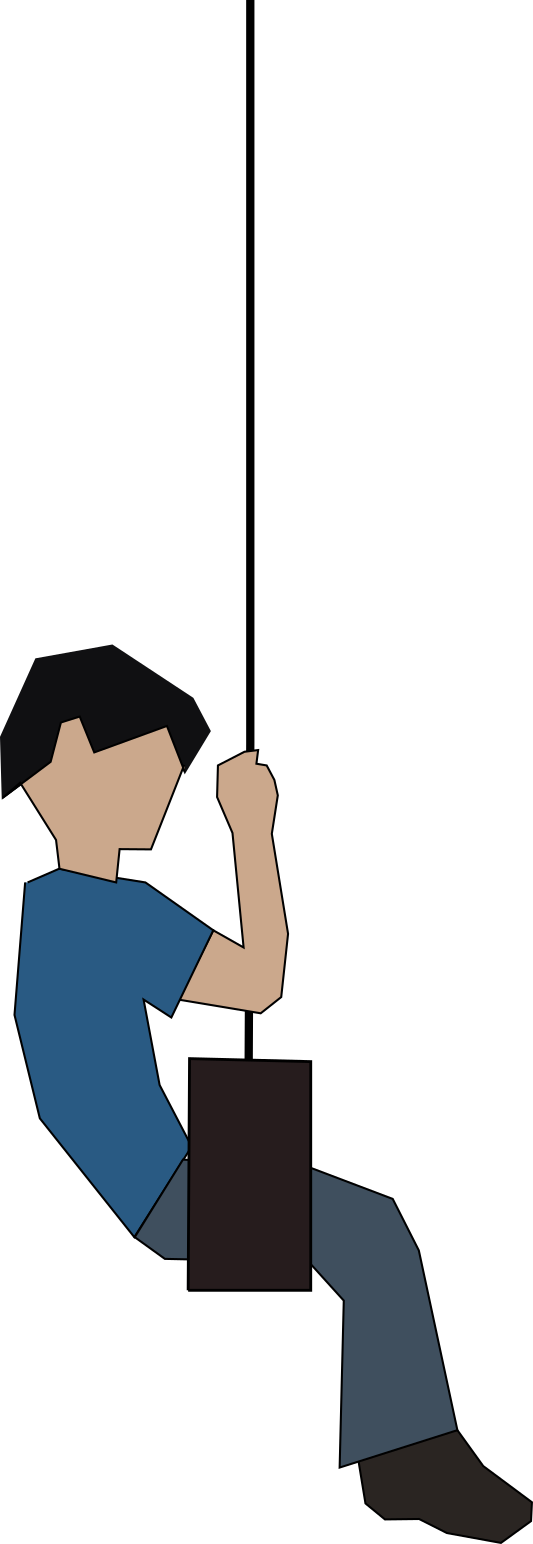
\includegraphics[width=0.5\textwidth]{/home/melanie/Work/pictures/physics/kind_schaukel.png}
\end{center}

\end{column}

\begin{column}{7cm}


\(\nu_1\), \(\nu_2\) gleich (oder Vielfache voneinander): \\
Die Schwingung wird verstärkt (Resonanz). \\[0.5 cm]

\pause

Im schlimmsten Fall: Resonanzkatastrophe!

\begin{center}
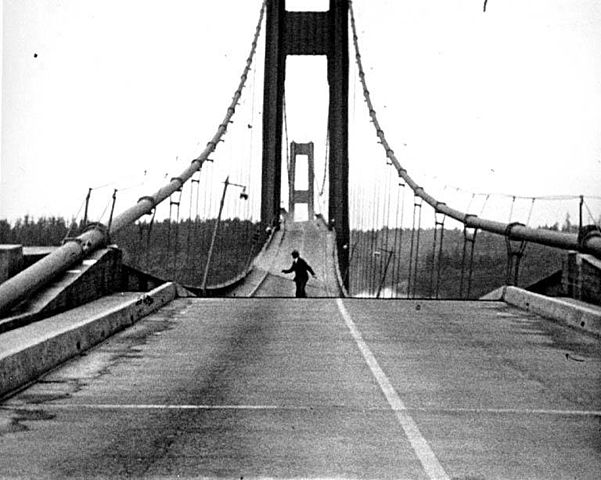
\includegraphics[width=0.8\textwidth]{/home/melanie/Work/pictures/physics/tacoma_bridge.jpg}
\end{center}

\end{column}

\end{columns}

\end{frame}




%% resonanz + Resonanzkatastrophe: Tacoma bridge collapse 


%%%%%%%%%%%%%%%%%%%%%%%%%%%%%%%%%%%
%% Wellen
%%%%%%%%%%%%%%%%%%%%%%%%%%%%%%%%%%%

\section{Wellen}



%% Definition einer Welle
\begin{frame}
\makebox[\linewidth]{\includegraphics[page=12,width=\textwidth]{Walter_Wellen.pdf}}
\end{frame}

%% Wellenlänge, Ausbreitungsgeschwindigkeit
\begin{frame}
  \frametitle{Ausbreitungsgeschwindigkeit = Wellenlänge mal Frequenz}

\[
c = \lambda \times f
\]

\begin{block}{Ausbreitungsgeschwindigkeiten}

\begin{tabular}{lr}
Licht (im Vakuum)       & \SI{300\,000\,000}{\meter\per\second} \\
Licht (im Wasser)       & \SI{230\,000\,000}{\meter\per\second} \\
Schall (in der Luft)    & \SI{330}{\meter\per\second} \\
Schall (im Wasser)      & \SI{1500}{\meter\per\second} \\
p-Wellen bei Erdbeben (in der Erdkruste)     & \SI{5000}{\meter\per\second} \\
\end{tabular}

\end{block}

\pause

Ausbreitungsgeschwindigkeit ist (pro Welle und Medium) konstant \\
\(\rightarrow\)  Je größer die Wellenlänge desto kleiner die Frequenz \\

\end{frame}

\begin{frame}
\frametitle{Schall vs Elektromagnetische Wellen}

\begin{tabular}{|l|l|l|}
\hline
        & \color{theme}{\textbf{Schallwellen}}  & \color{theme}{\textbf{Elektromagnetische Wellen}}     \\
\hline
Ausbreitung       & \SI{330}{\meter\per\second} (Luft)  &  \(\sim\)\SI{300\,000\,000}{\meter\per\second} (Vakuum)   \\
\hline
\end{tabular}
\end{frame}


\begin{frame}
\frametitle{Wie weit ist das Gewitter weg?}

\begin{columns}[c]

\begin{column}{5cm}

\begin{center}
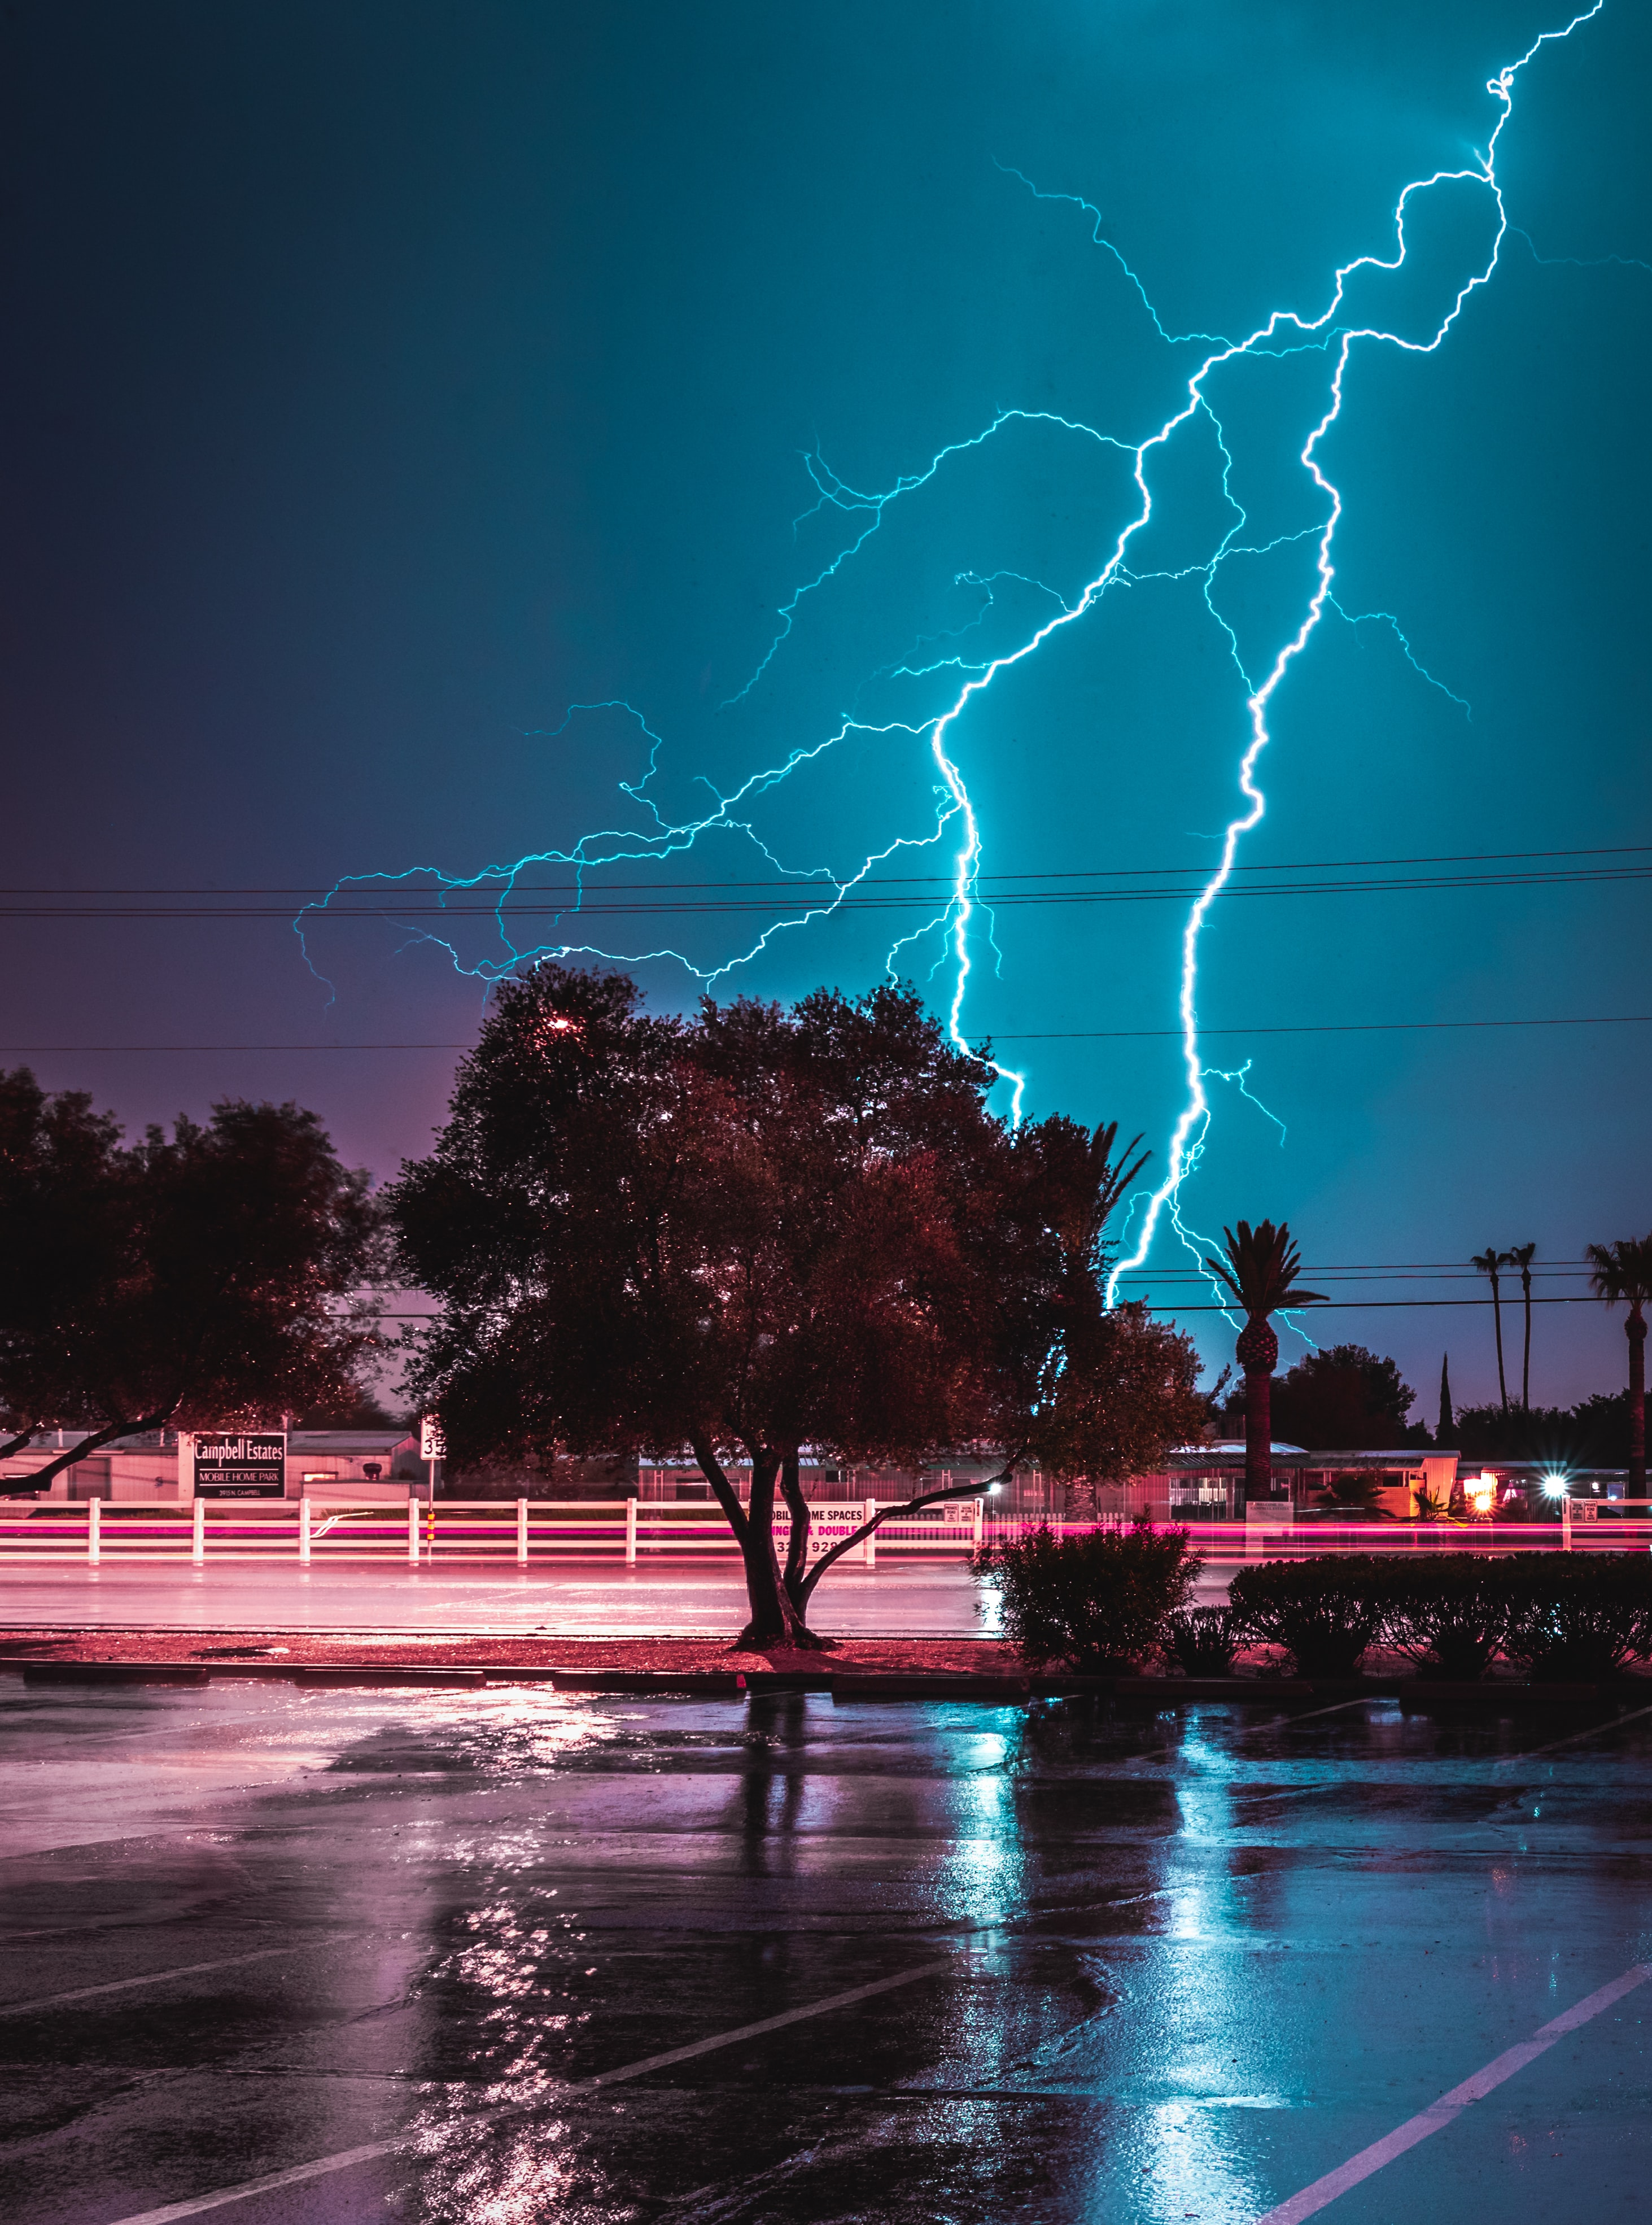
\includegraphics[width=\textwidth]{/home/melanie/Work/pictures/physics/gewitter.jpg}
\end{center}



\end{column}

\begin{column}{5cm}

\begin{itemize}
\item
Beginne beim Blitz zu zählen (Sekunden)
\item
Zähle, bis der Donner kommt
\item
Dividiere die Zahl durch 3
\item
So viele Kilometer ist das Gewitter entfernt
\item
\textcolor{theme}{Warum funktioniert das?}
\end{itemize}


\end{column}

\end{columns}


\end{frame}


%% Longitudinal- und Transversalwellen


%%%%% Definition
\begin{frame}
\frametitle{Wellenrichtung}

Bei Transversalwellen steht die Wellenrichtung senkrecht zur Ausbreitungsrichtung. \\

\begin{center}
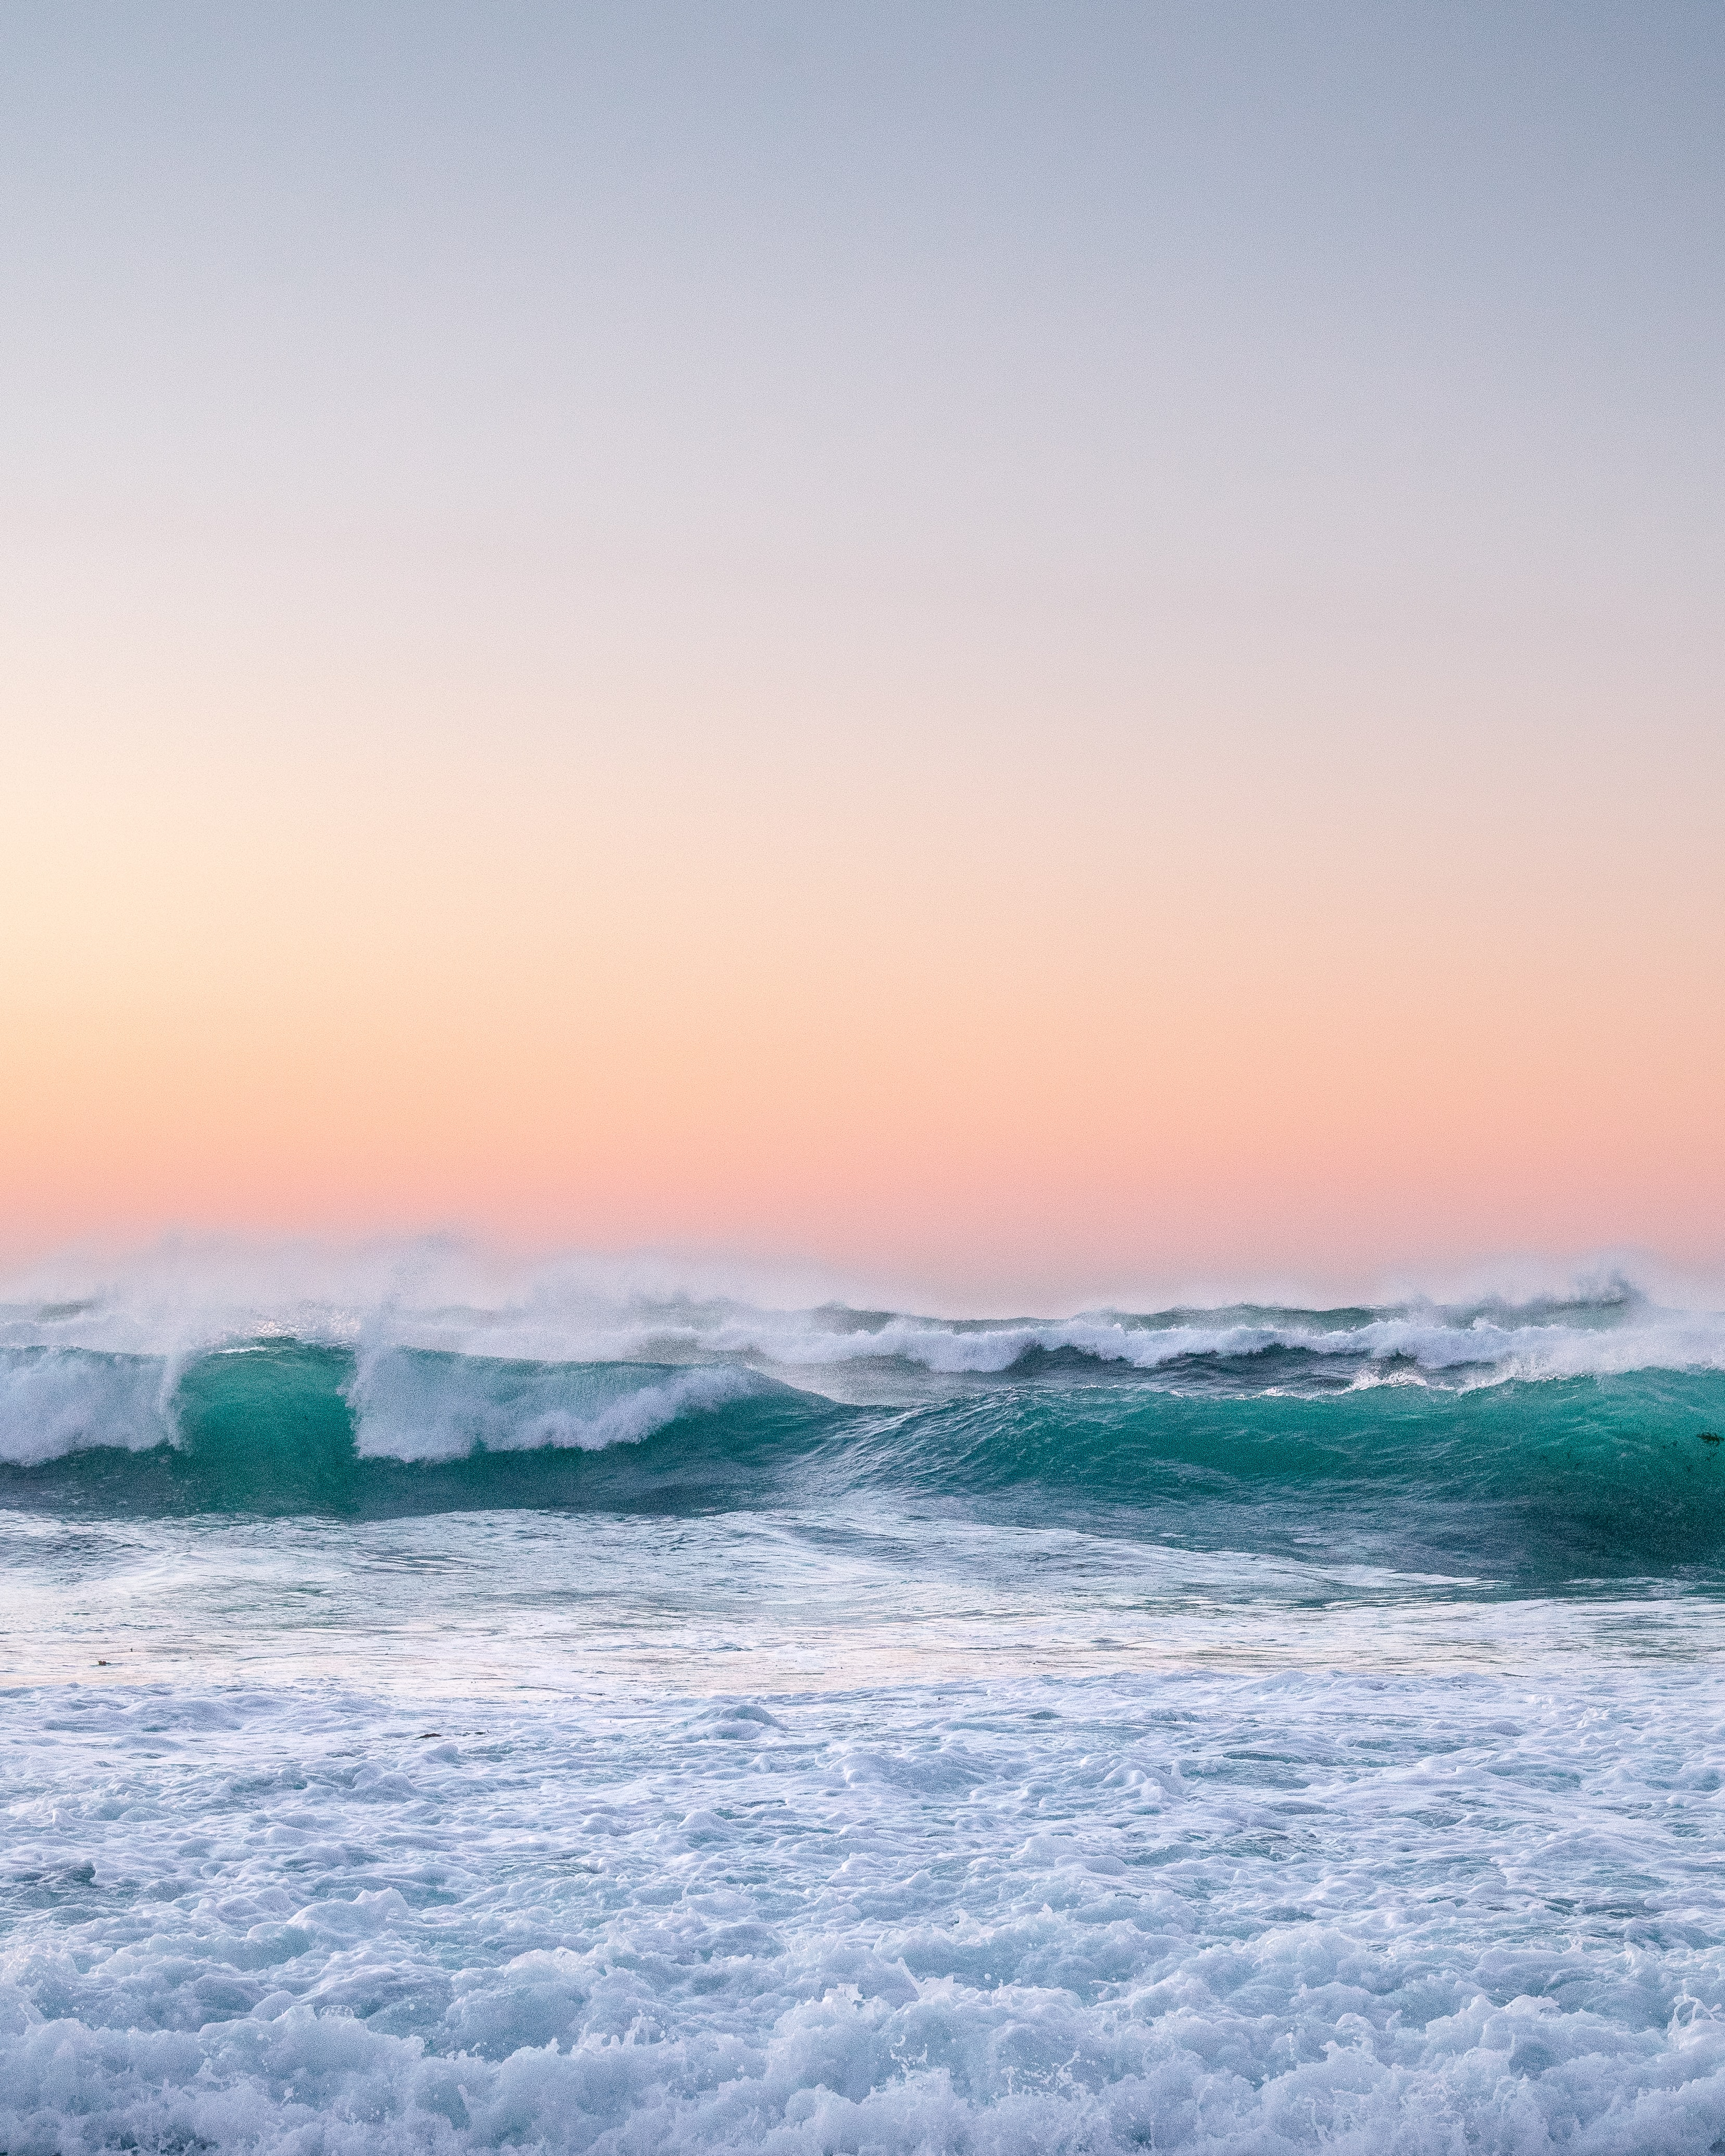
\includegraphics[width=0.4\textwidth]{/home/melanie/Work/pictures/physics/wellen_meer.jpg}
\end{center} 


\end{frame}

\begin{frame}
\frametitle{Wellenrichtung}

Bei Longitudinalwellen ist die Wellenrichtung die Ausbreitungsrichtung. 

\begin{center}
\includegraphics[width=0.6\textwidth]{/home/melanie/Work/pictures/animals/regenwurm.jpg}
\end{center}

\end{frame}



\begin{frame}
\frametitle{Wellenrichtung}
Schallwellen sind Longitudinalwellen, elektromagnetische Wellen (z.B. Licht) sind Transversalwellen \\[1cm]

\pause

\begin{tabular}{|l|l|l|}
\hline
        & \color{theme}{\textbf{Schallwellen}}  & \color{theme}{\textbf{Elektromagnetische Wellen}}     \\
\hline
Ausbreitung       & \SI{330}{\meter\per\second} (Luft)  &  \(\sim\)\SI{300\,000\,000}{\meter\per\second} (Vakuum)   \\
\hline
Richtung        & Longitudinal  & Transversal   \\
\hline
\end{tabular}

\end{frame}





%% Doppler Effect

\begin{frame}
\frametitle{Frage}

\begin{columns}[c]

\begin{column}{5cm}
\begin{center}
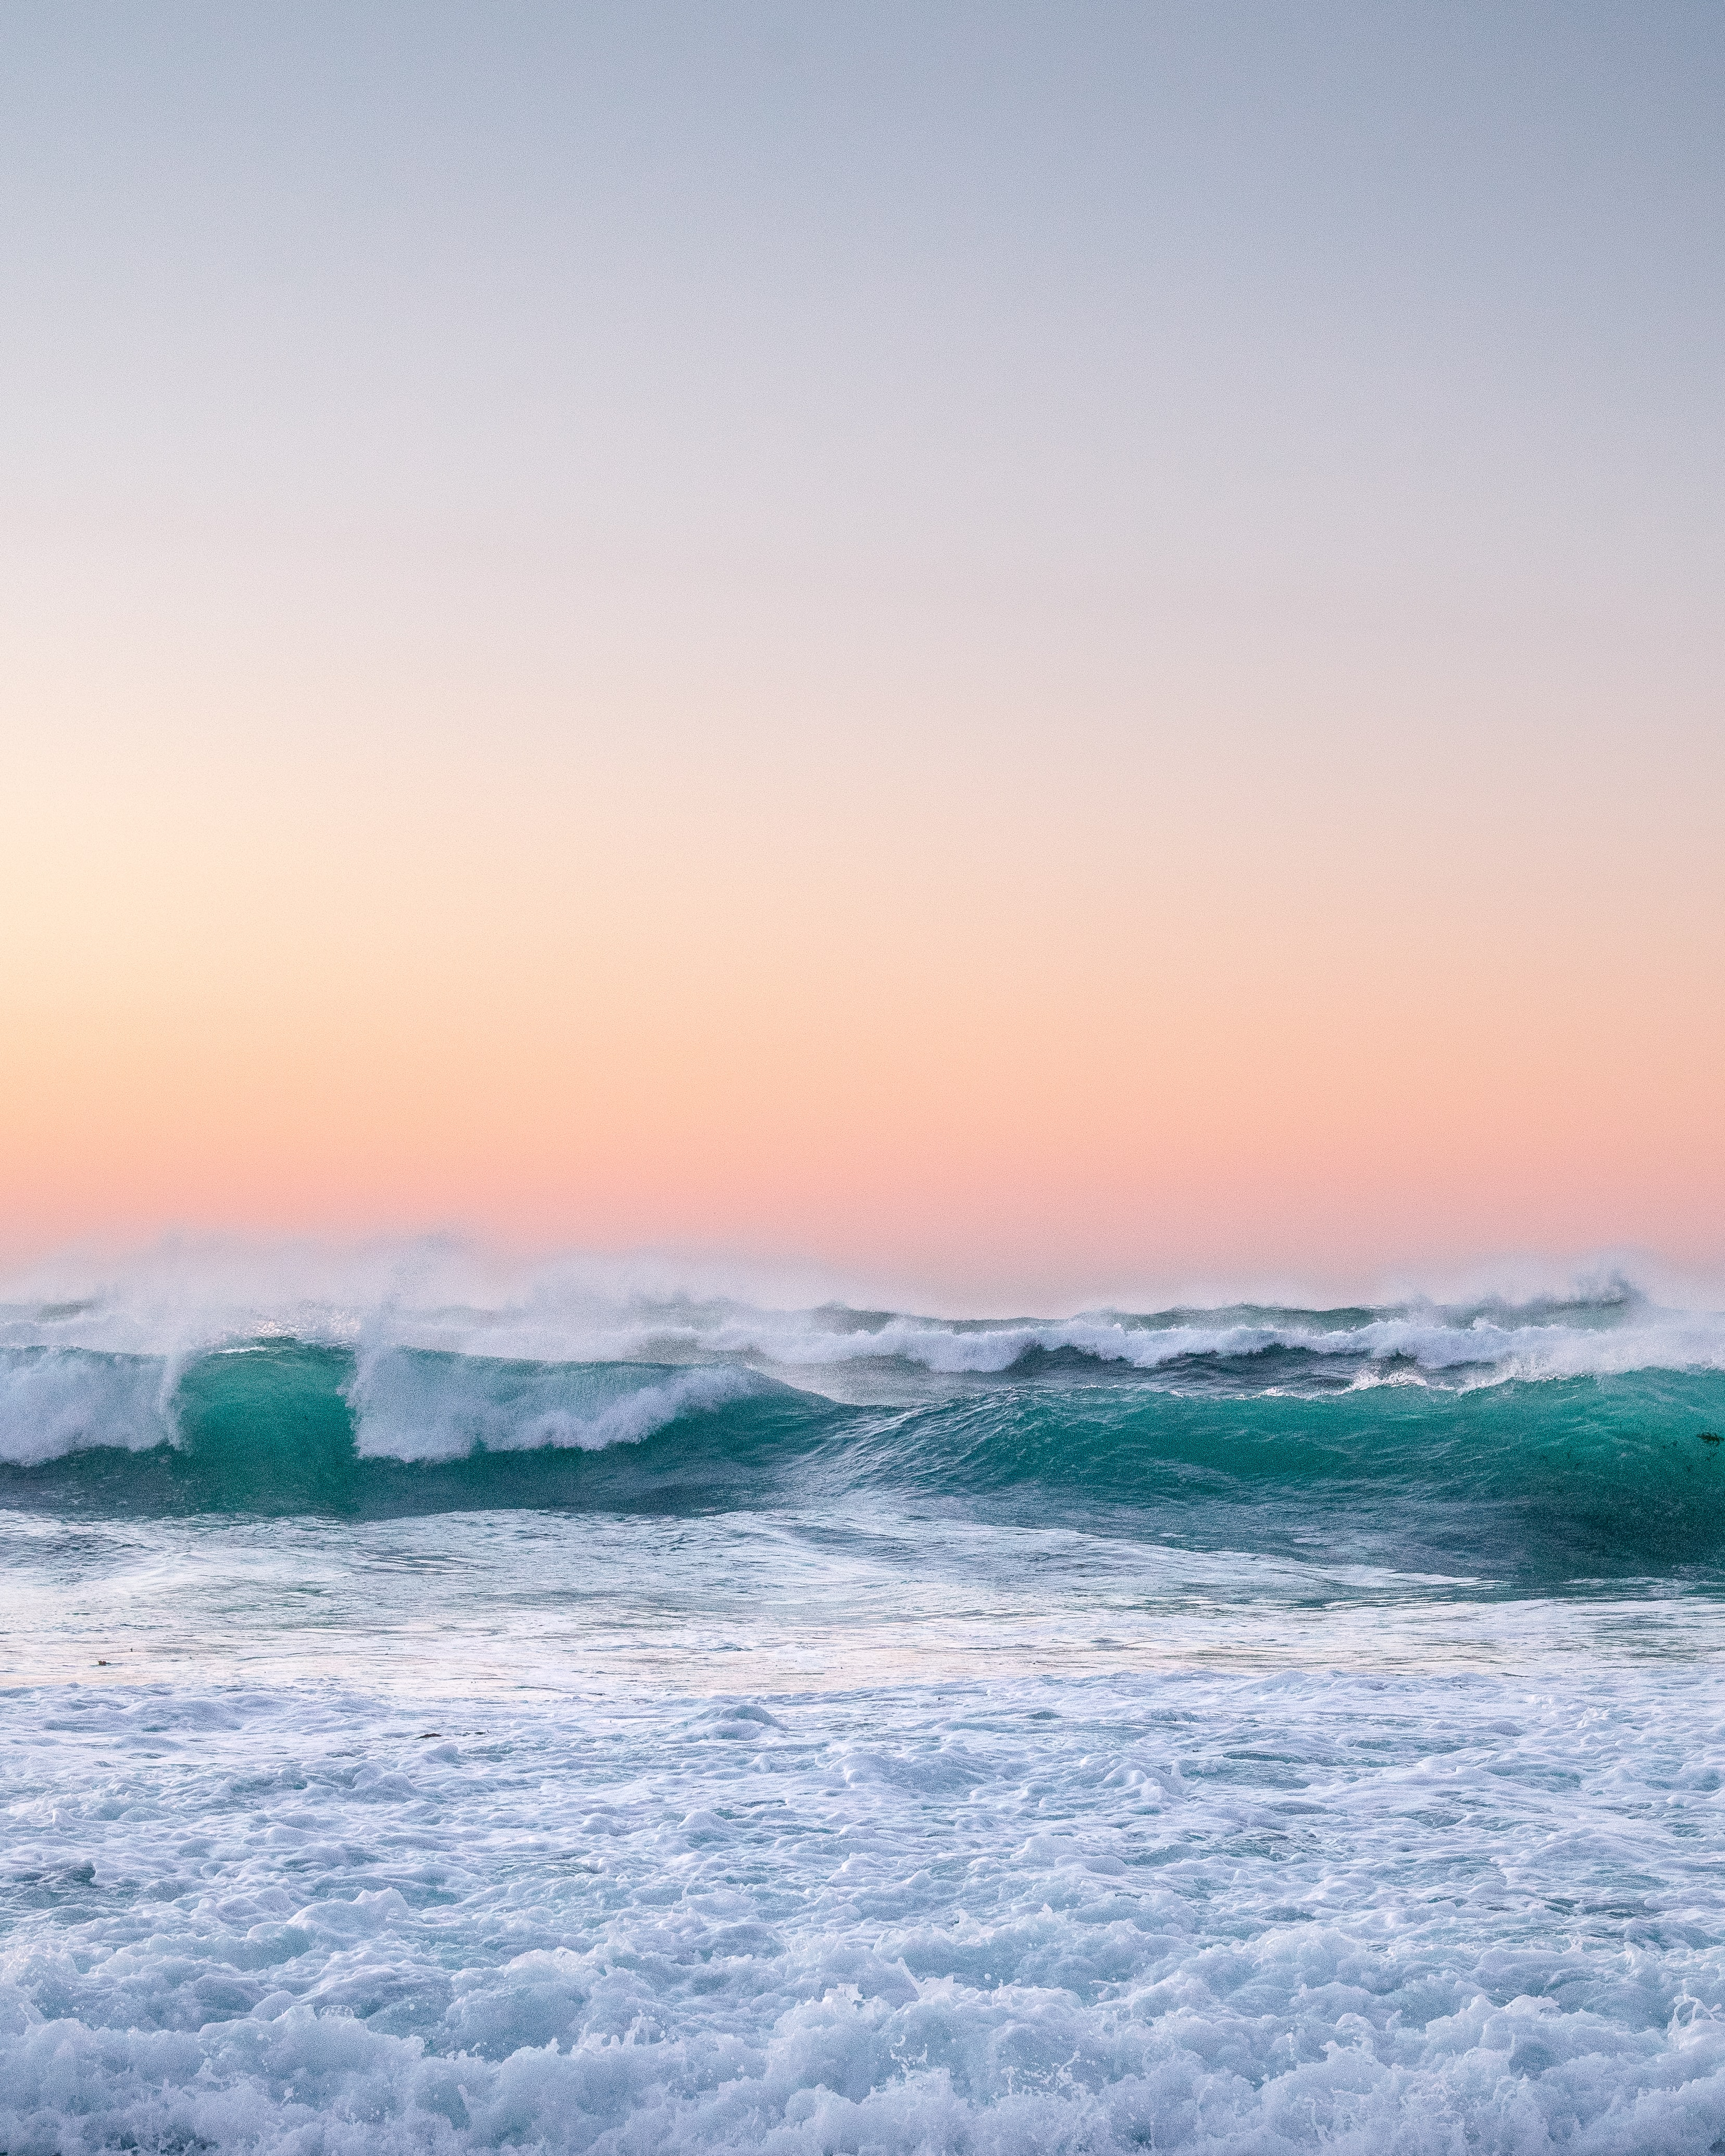
\includegraphics[width=\textwidth]{/home/melanie/Work/pictures/physics/wellen_meer.jpg}
\end{center}

\end{column}


\begin{column}{5cm}

Eine Welle kommt alle 7 Sekunden. \\[0.5 cm]

Wie oft begegnen Sie einer Welle, wenn Sie


\begin{itemize}
\item
Den Wellen entgegen schwimmen?
\item
In die andere Richtung schwimmen?
\end{itemize}


\end{column}


\end{columns}

\end{frame}




\begin{frame}
\frametitle{Doppler Effekt}

Frequenzen erscheinen höher, wenn wir uns auf die Quelle einer Wellenbewegung zu bewegen (oder sie auf uns). Frequenzen erscheinen geringer, wenn wir uns von der Quelle wegbewegen. 


\begin{columns}[c]

\pause

\begin{column}{5cm}

Beispiel: Doppler-Sonographie \\

Ultraschall-Anwendung. Verschiebung der Frequenz lässt Rückschlüsse darauf zu, in welche Richtung und wie schnell sich z.B. Blut in einem Gewebe bewegt.


\end{column}

\begin{column}{5cm}
\begin{center}
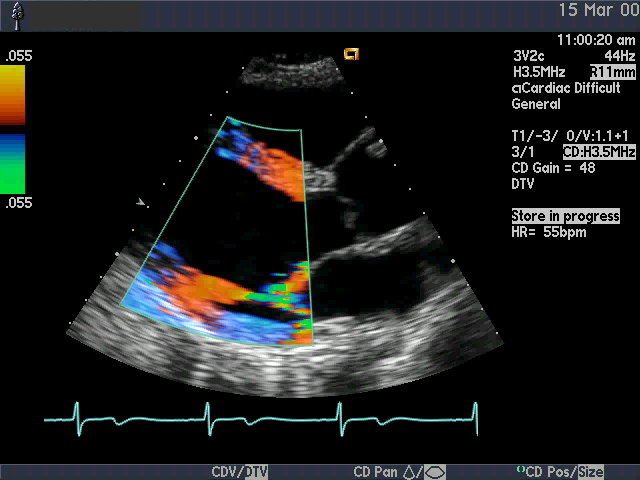
\includegraphics[width=\textwidth]{/home/melanie/Work/pictures/physics/Tissue_Doppler.png}
\end{center}
\end{column}

\end{columns}

\end{frame}




%% Interferenz + Schwebung + Noise cancelling headphones
\begin{frame}
\frametitle{Was passiert, wenn sich zwei Wellen überlagern?}

\begin{columns}[c]

\begin{column}{5cm}

\begin{center}
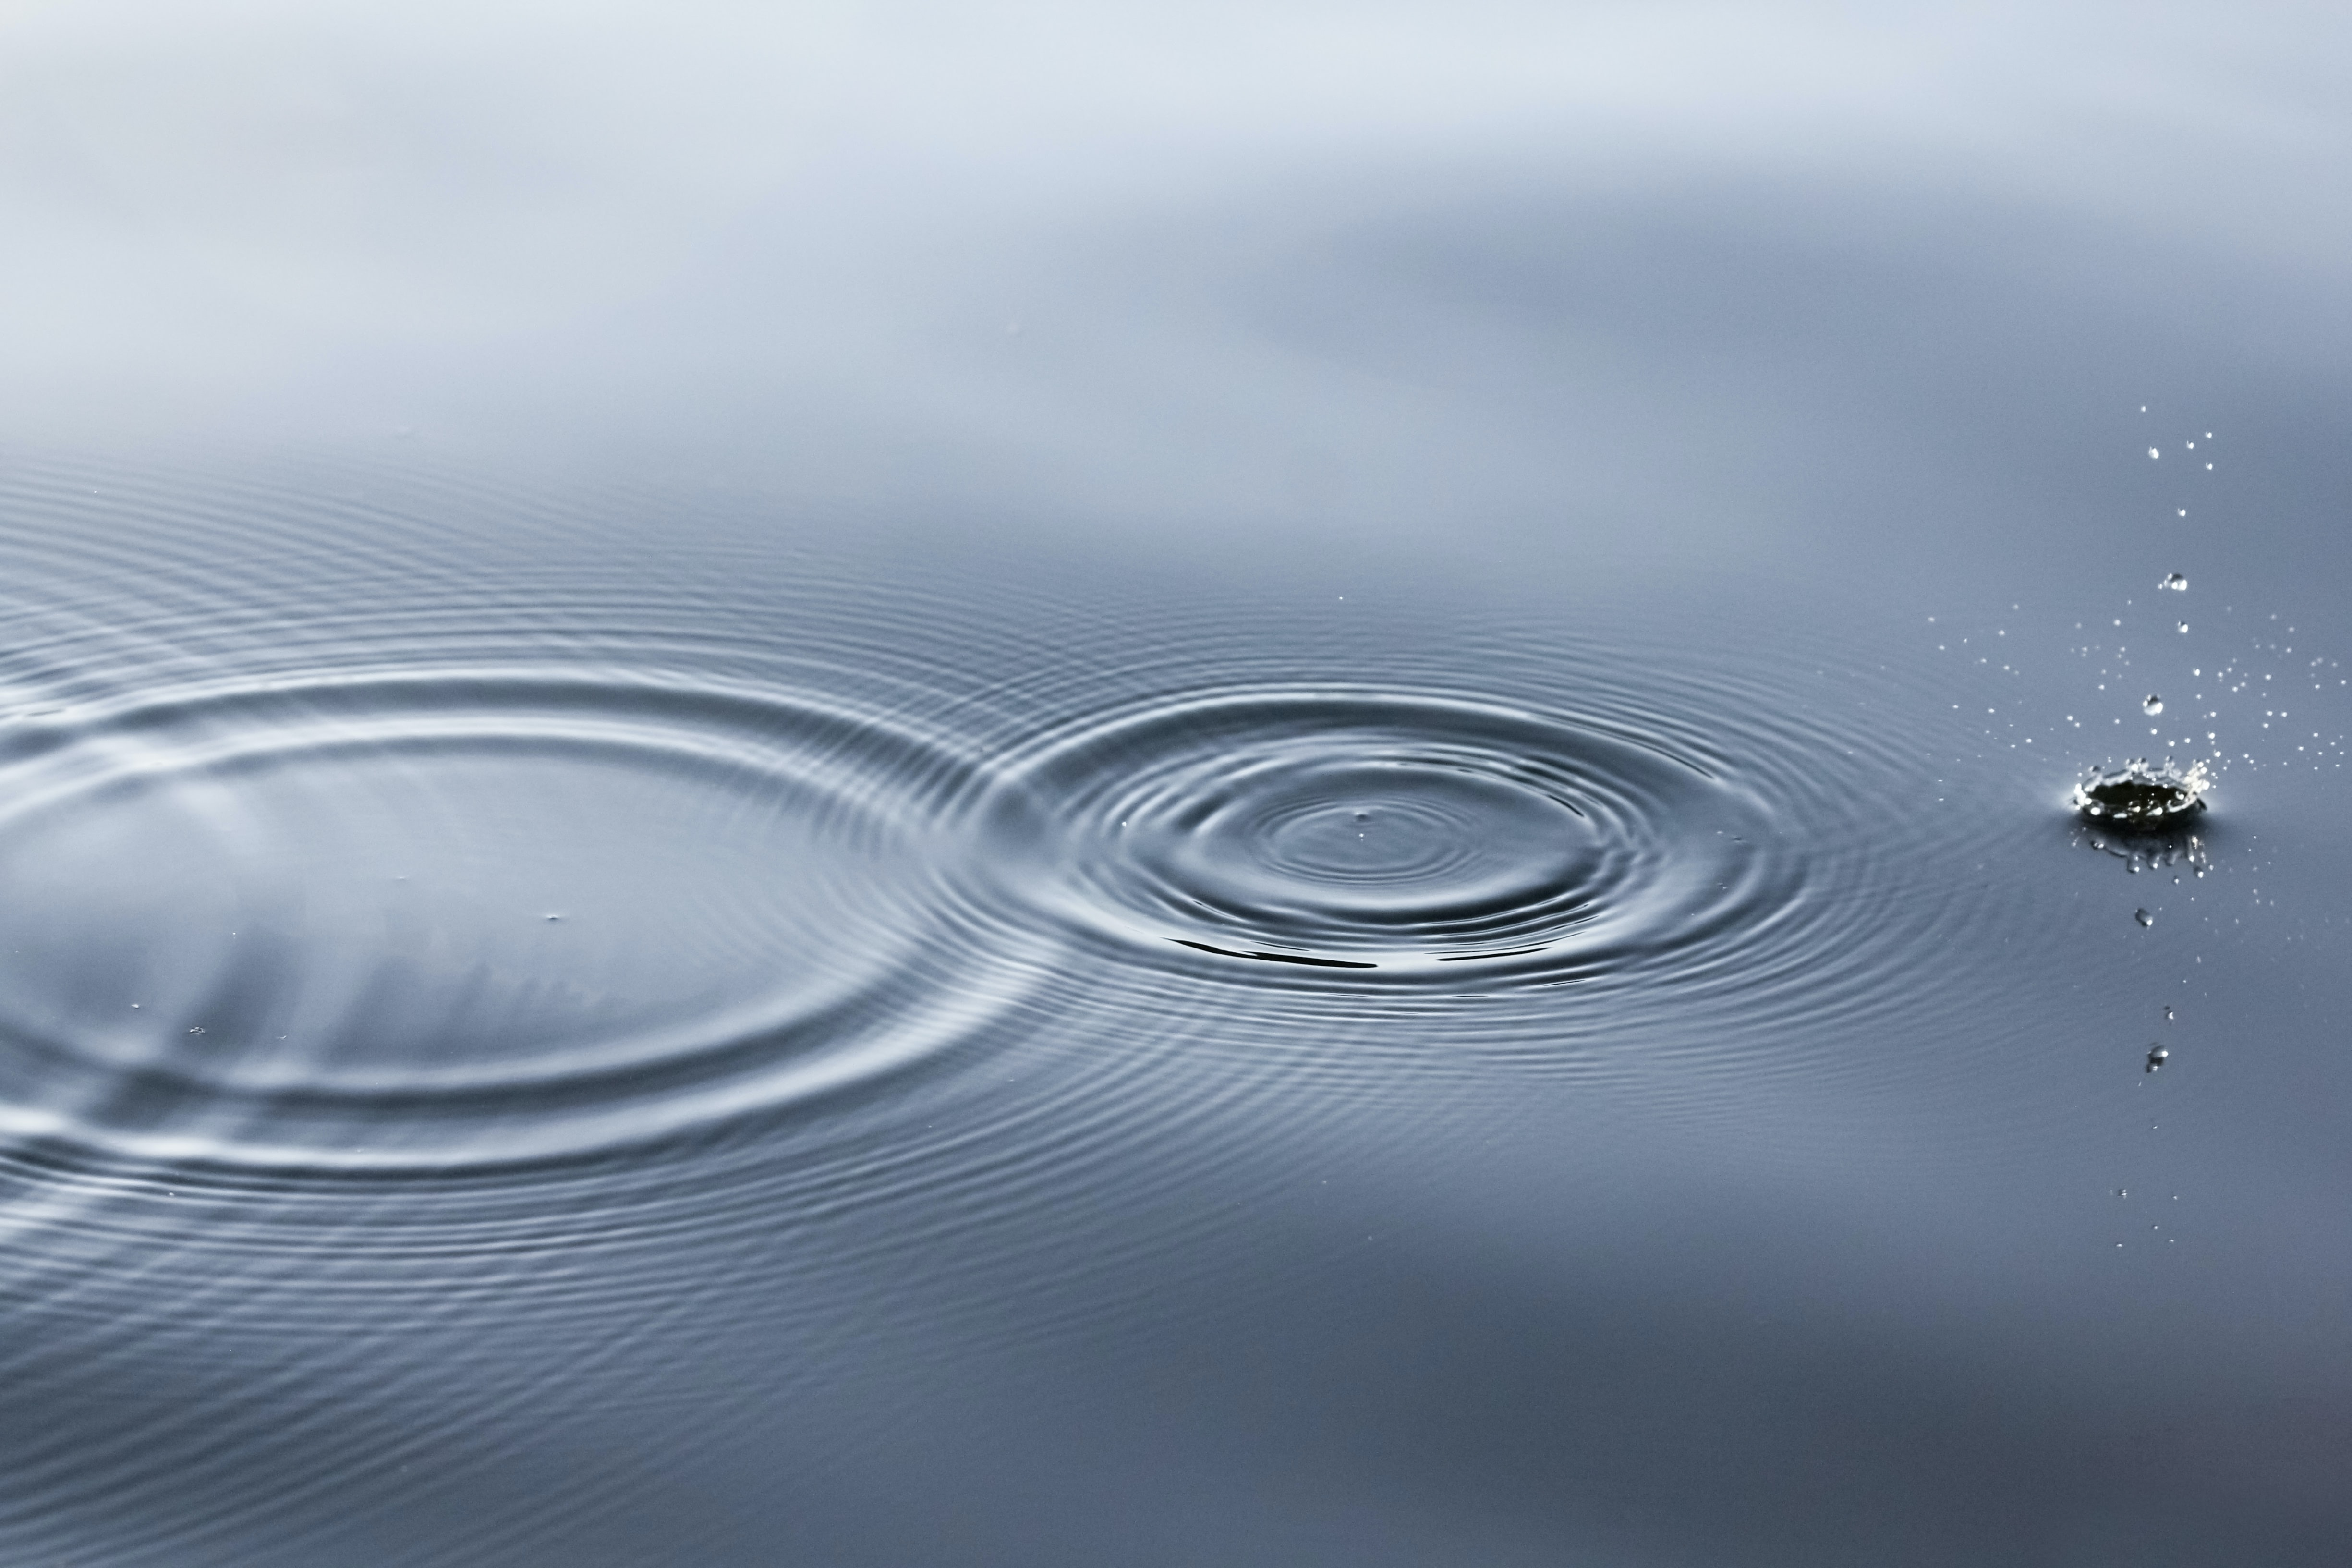
\includegraphics[width=\textwidth]{/home/melanie/Work/pictures/physics/wellen.jpg}
\end{center}


\end{column}

\pause

\begin{column}{5cm}

\begin{itemize}
\item
Bei Wellen unterschiedlicher Frequenz:  Schwebung
\item
Bei Wellen gleicher Frequenz: Interferenz 

\end{itemize}


\end{column}

\end{columns}


\end{frame}



\begin{frame}
\makebox[\linewidth]{\includegraphics[page=19,width=\textwidth]{Walter_Wellen.pdf}}
\end{frame}

\begin{frame}
\makebox[\linewidth]{\includegraphics[page=15,width=\textwidth]{Walter_Wellen.pdf}}
\end{frame}


\begin{frame}
\frametitle{Interferenz: Anwendung}

\begin{columns}[c]

\begin{column}{5cm}
\begin{center}
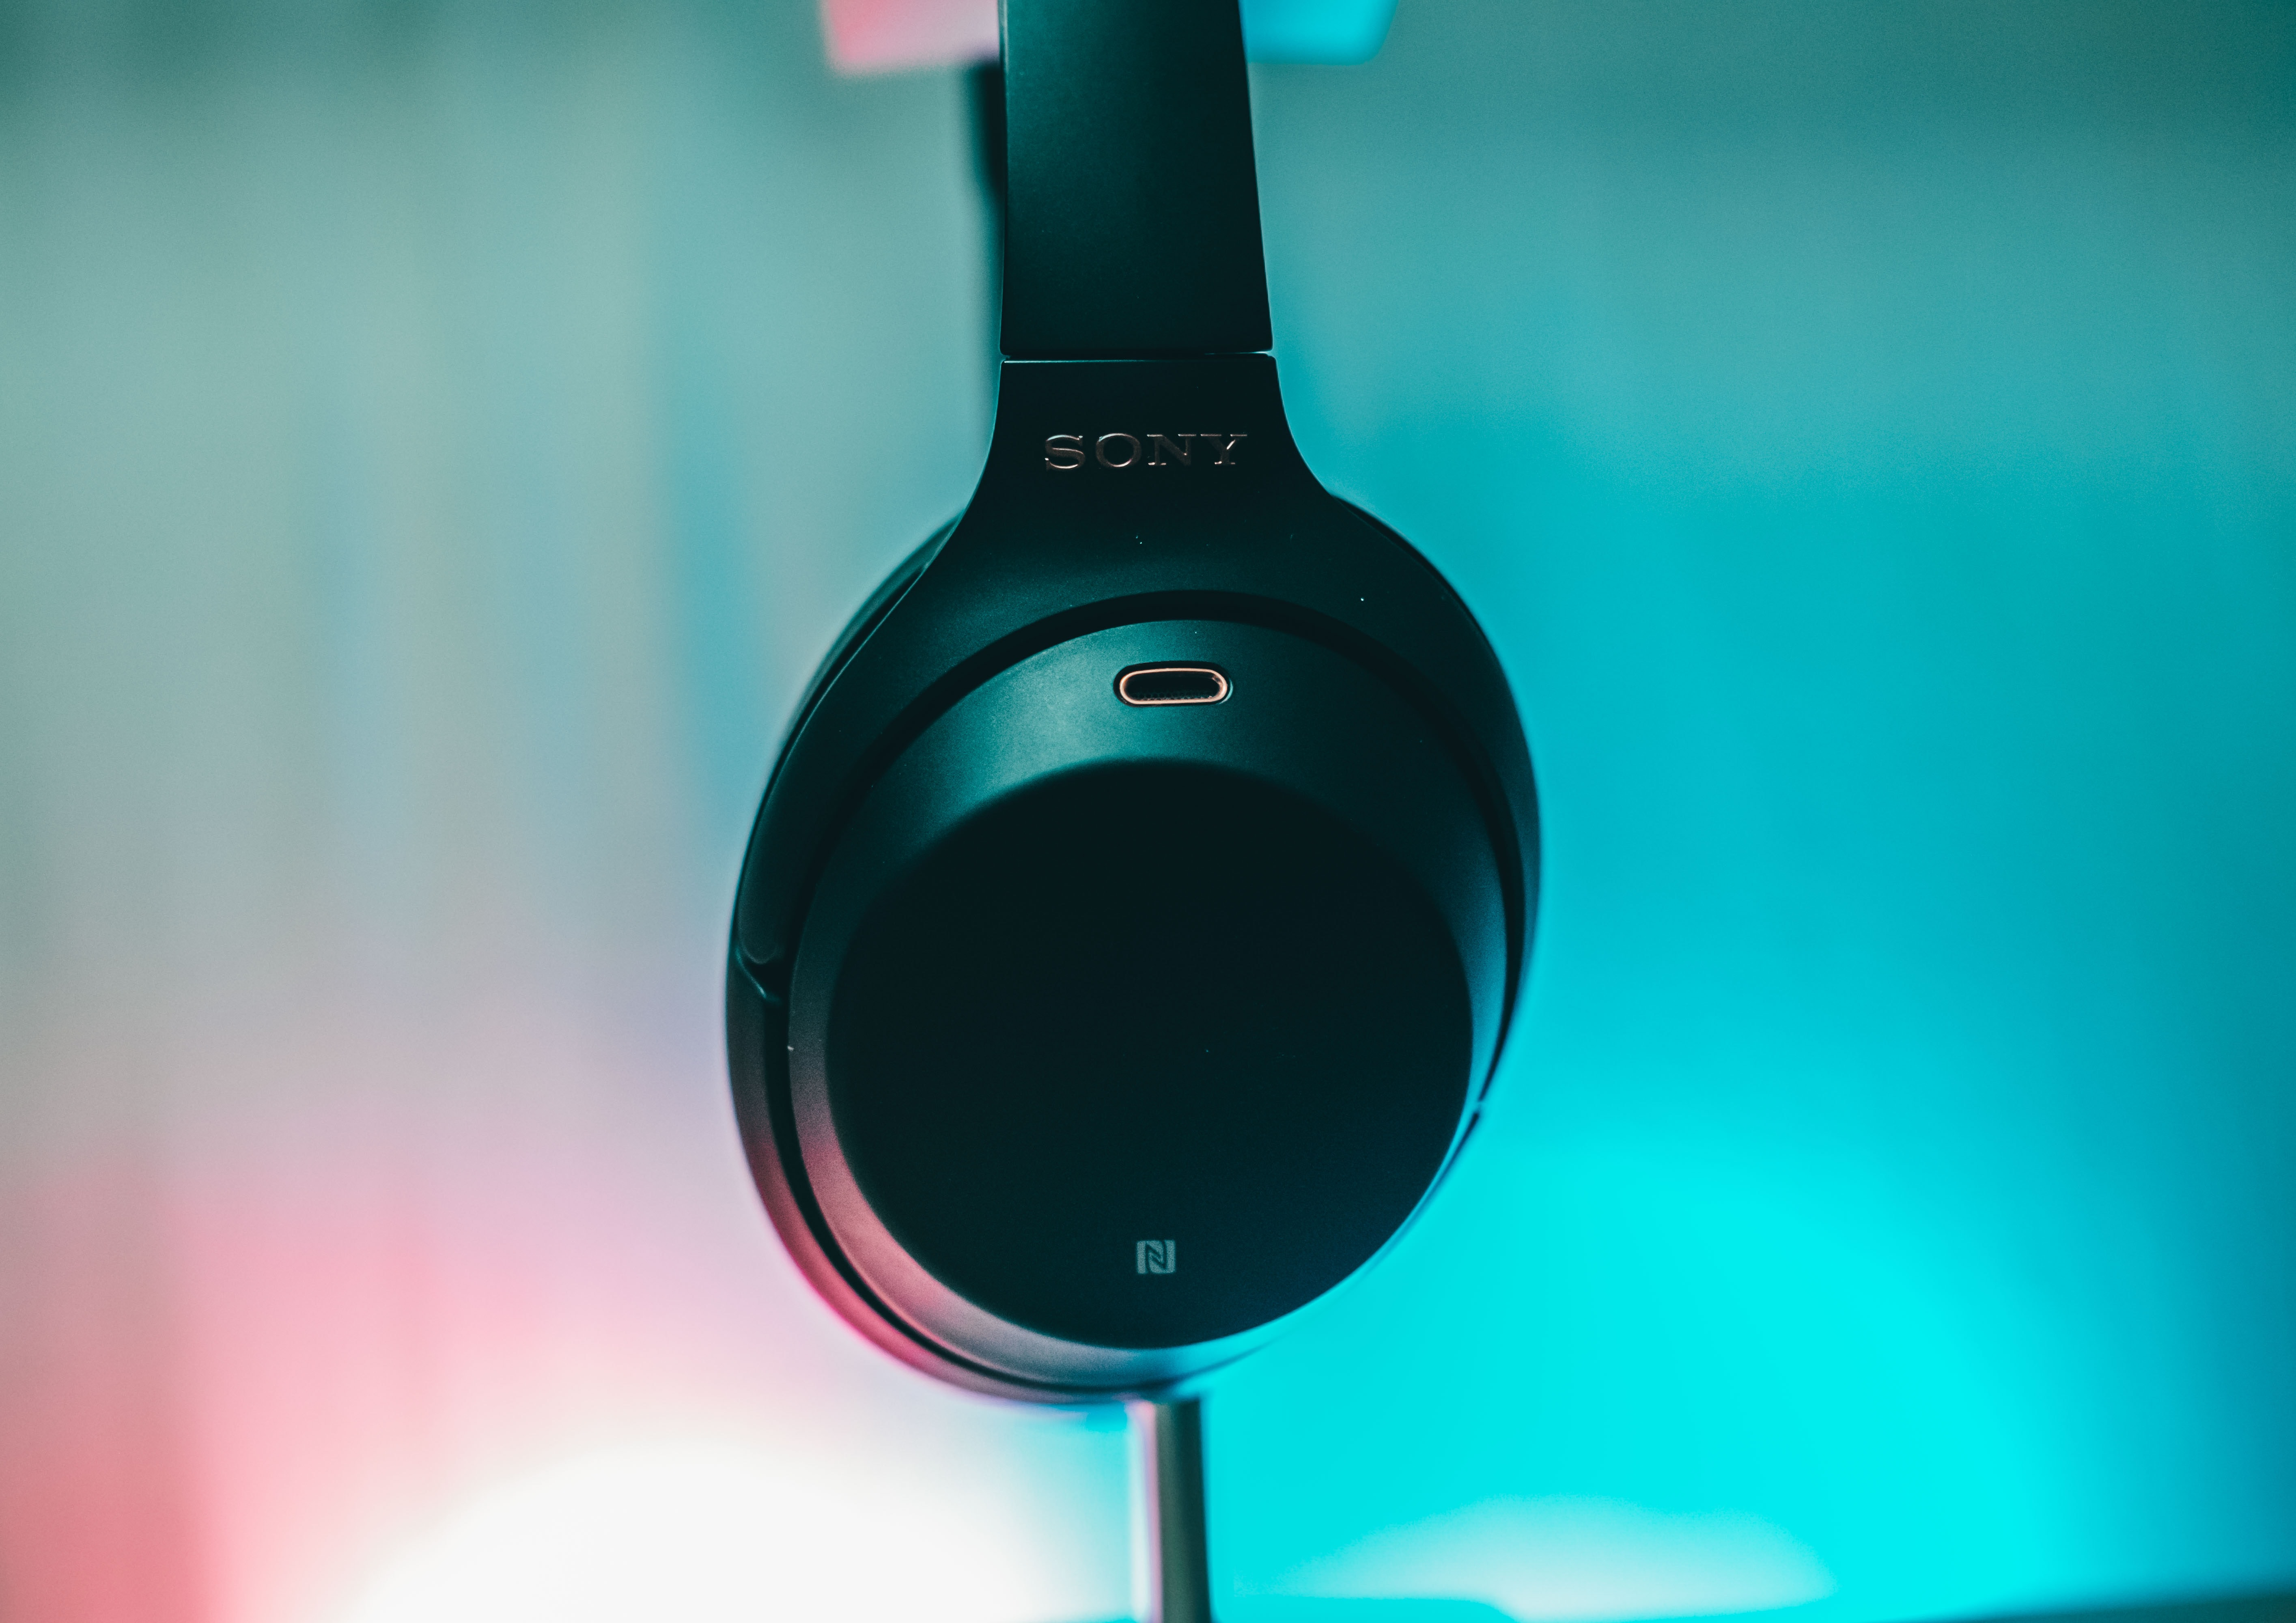
\includegraphics[width=\textwidth]{/home/melanie/Work/pictures/physics/noise_cancelling_headphones.jpg}
\end{center}
\end{column}

\begin{column}{5cm}

\begin{block}{Noise-cancelling Kopfhörer:}

\begin{itemize}
\item 
Nehmen die Schallwellen aus der Umgebung auf 
\item
Berechnen die Schallwellen, die nötig sind, um eine destruktive Interferenz zu erzeugen
\item
Spielen genau diese Schallwellen aus einem kleinen Mikrofon.
\end{itemize}


\end{block}

\end{column}


\end{columns}

\end{frame}

%% Umkekehrt: Welche Wellen wurden hier überlagert?


%% Fourieranaylse
\begin{frame}
\frametitle{Fourieranalyse: Idee}


\begin{itemize}
\item
Jede komplexe Wellenform kann im Prinzip als Überlagerung von Sinuswellen verschiedener Frequenzen dargestellt werden
\item
Manchmal interessiert uns, welche Frequenzen wieviel zur Wellenform beitragen
\item
Dafür möchten wir eine Darstellung ``im Frequenzraum'' (statt Zeit stellen wir Frequenz auf der x-Achse dar)
\item
Die Fourier-Analyse leistet mathematisch genau das  
\item
Die Fourier-Synthese ist der umgekehrte Prozess
\end{itemize}


\end{frame}



%% Fourieranaylse
\begin{frame}
\frametitle{Fourieranalyse: Illustration}

\centering
\animategraphics[loop]{5}{/home/melanie/Work/pictures/physics/fourier}{1}{93}

\end{frame}

\begin{frame}
\frametitle{Fourieranalyse: Anwendung}

\begin{columns}[c]

\begin{column}{5cm}
\begin{block}{Datenkompression\\ (z.B. mp3)}

\begin{itemize}
\item
Fourier-Analyse zur Ermittlung des Frequenz-Spektrums
\item
Herausschneiden von unwichtigen* (z.B. nicht hörbaren) Frequenzen
\item
Dadurch wird das Datenvolumen verringert
\end{itemize}

\end{block}

\end{column}


\begin{column}{5cm}

\begin{center}
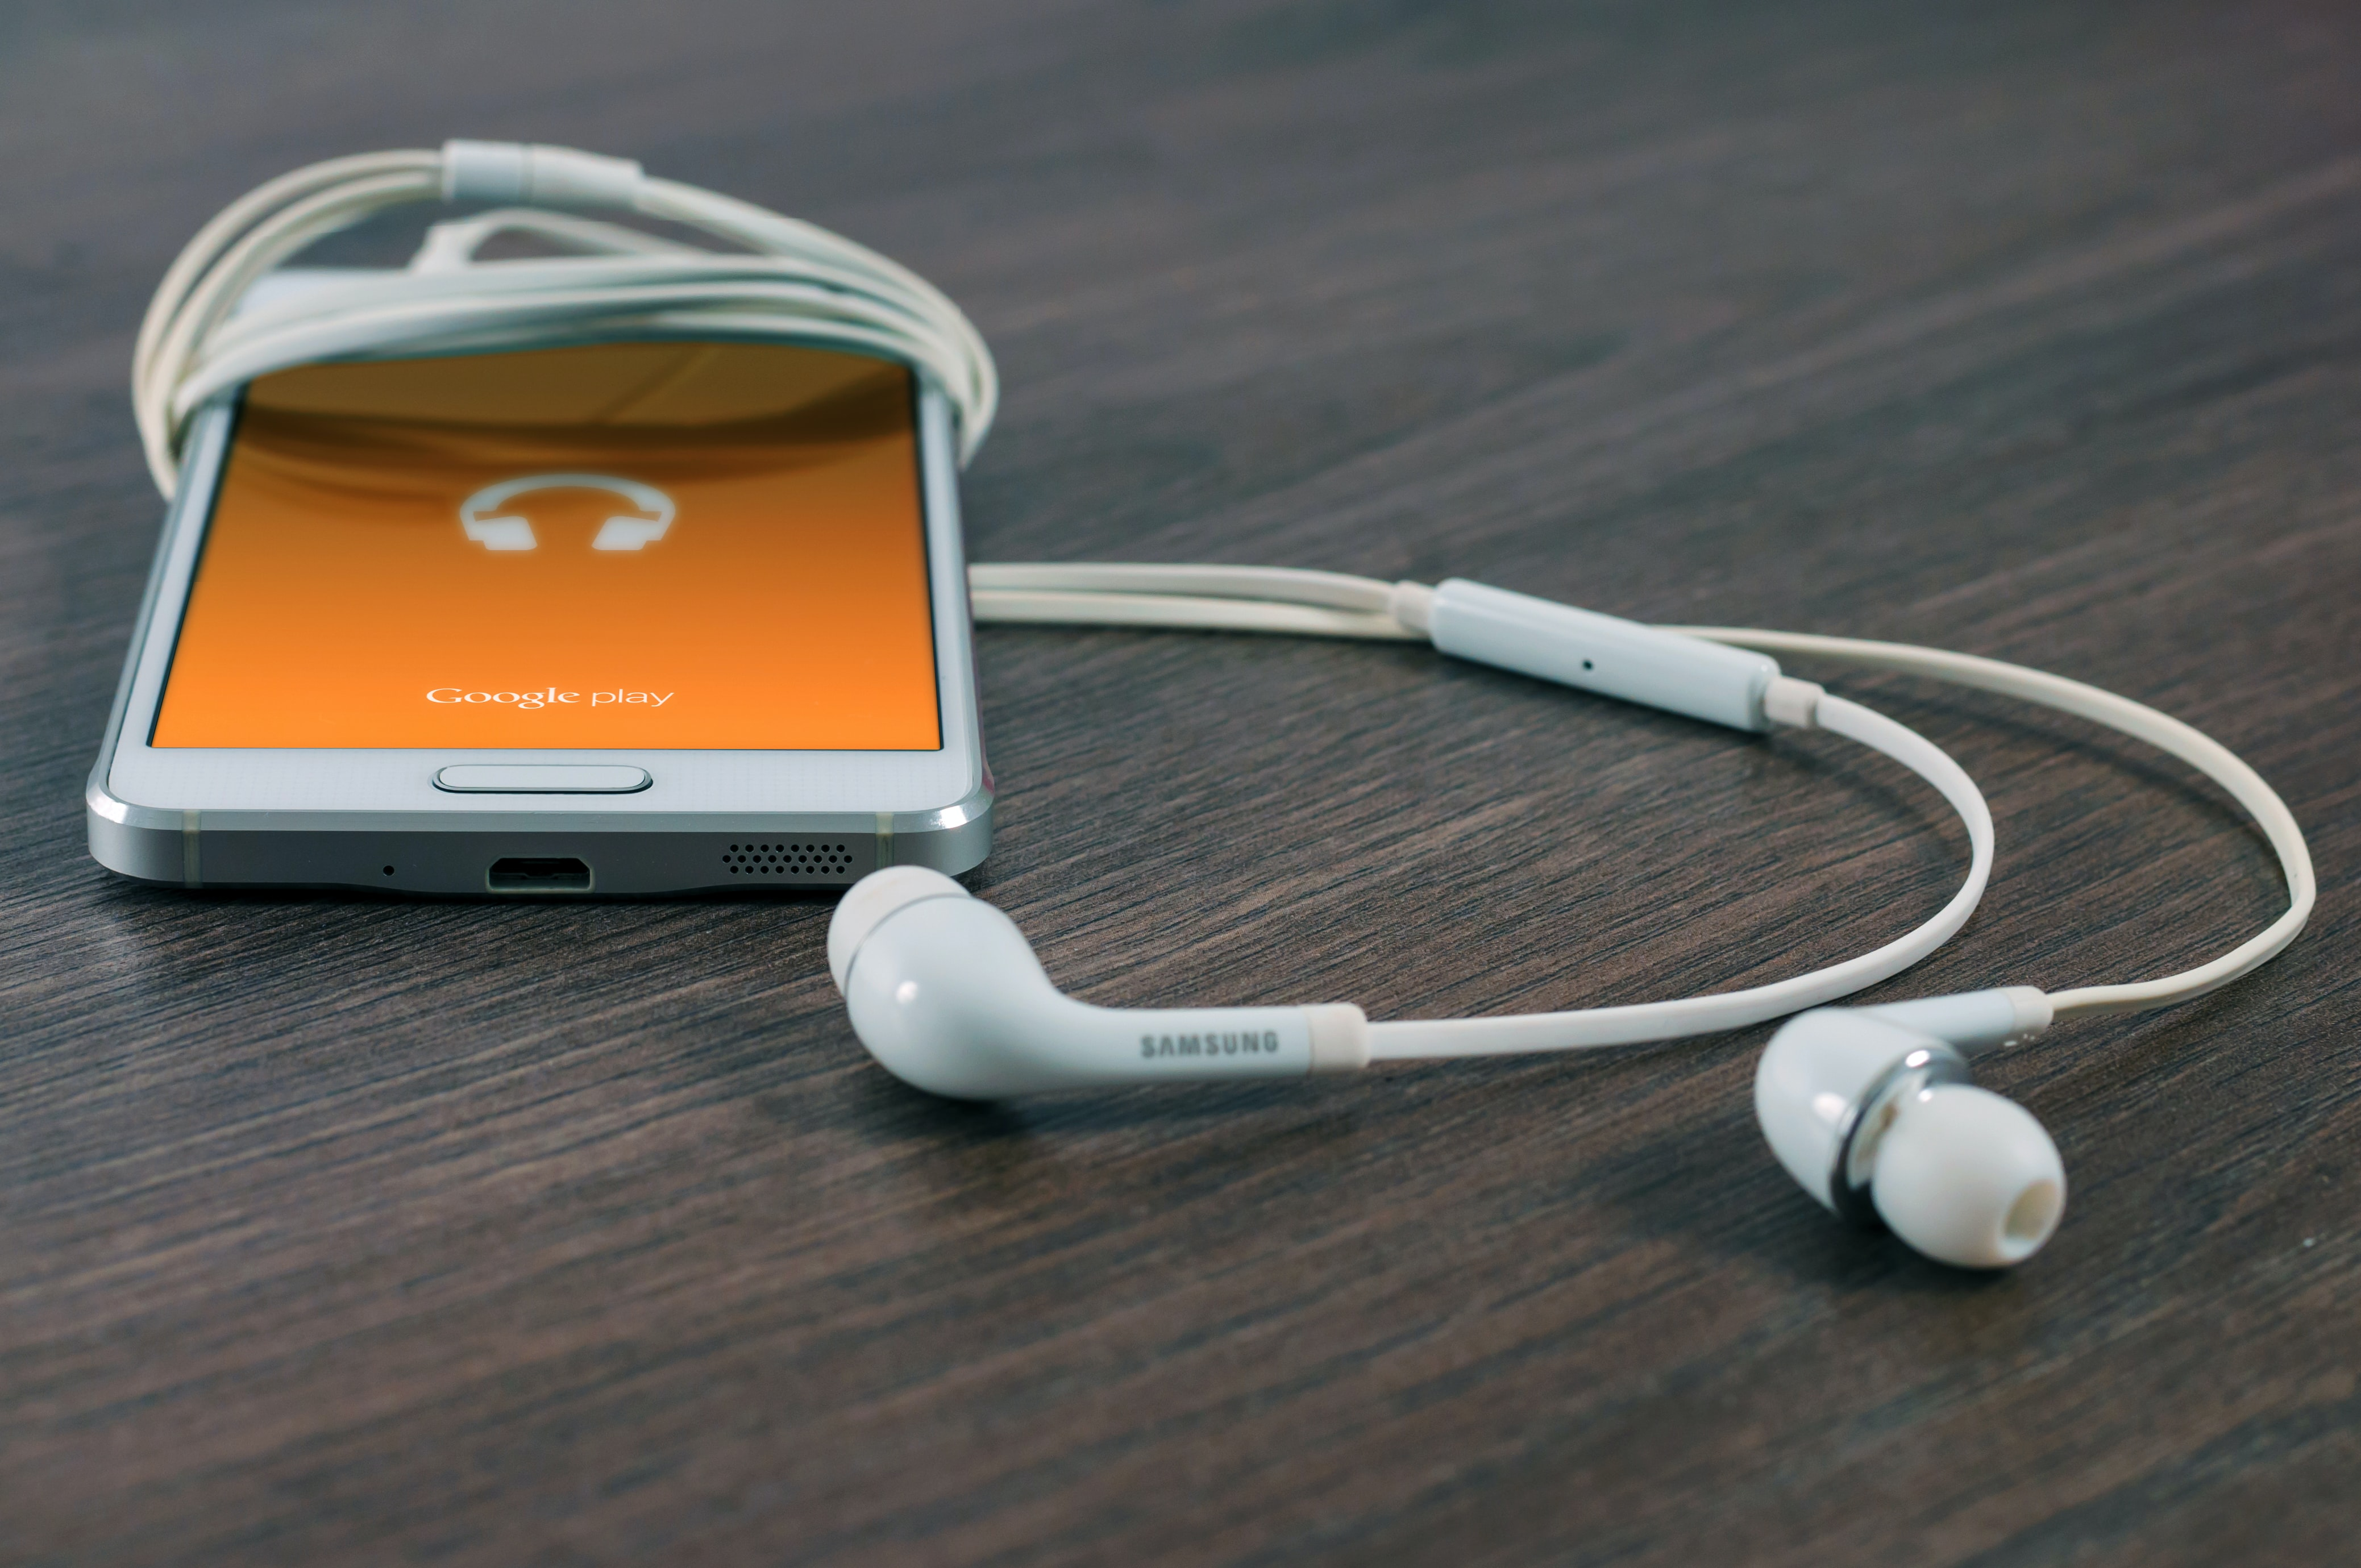
\includegraphics[width=\textwidth]{/home/melanie/Work/pictures/physics/phone_music.jpg}
\end{center}

\end{column}

\end{columns}


\end{frame}




%%%%%%%%%%%%%%%%%%%%%%%%%%%%%%%%%%%
%% Schallwellen
%%%%%%%%%%%%%%%%%%%%%%%%%%%%%%%%%%%

\section{Schall}

%% Schallwellen Definition
\begin{frame}
\makebox[\linewidth]{\includegraphics[page=26,width=\textwidth]{Walter_Wellen.pdf}}
\end{frame}


{
  \usebackgroundtemplate{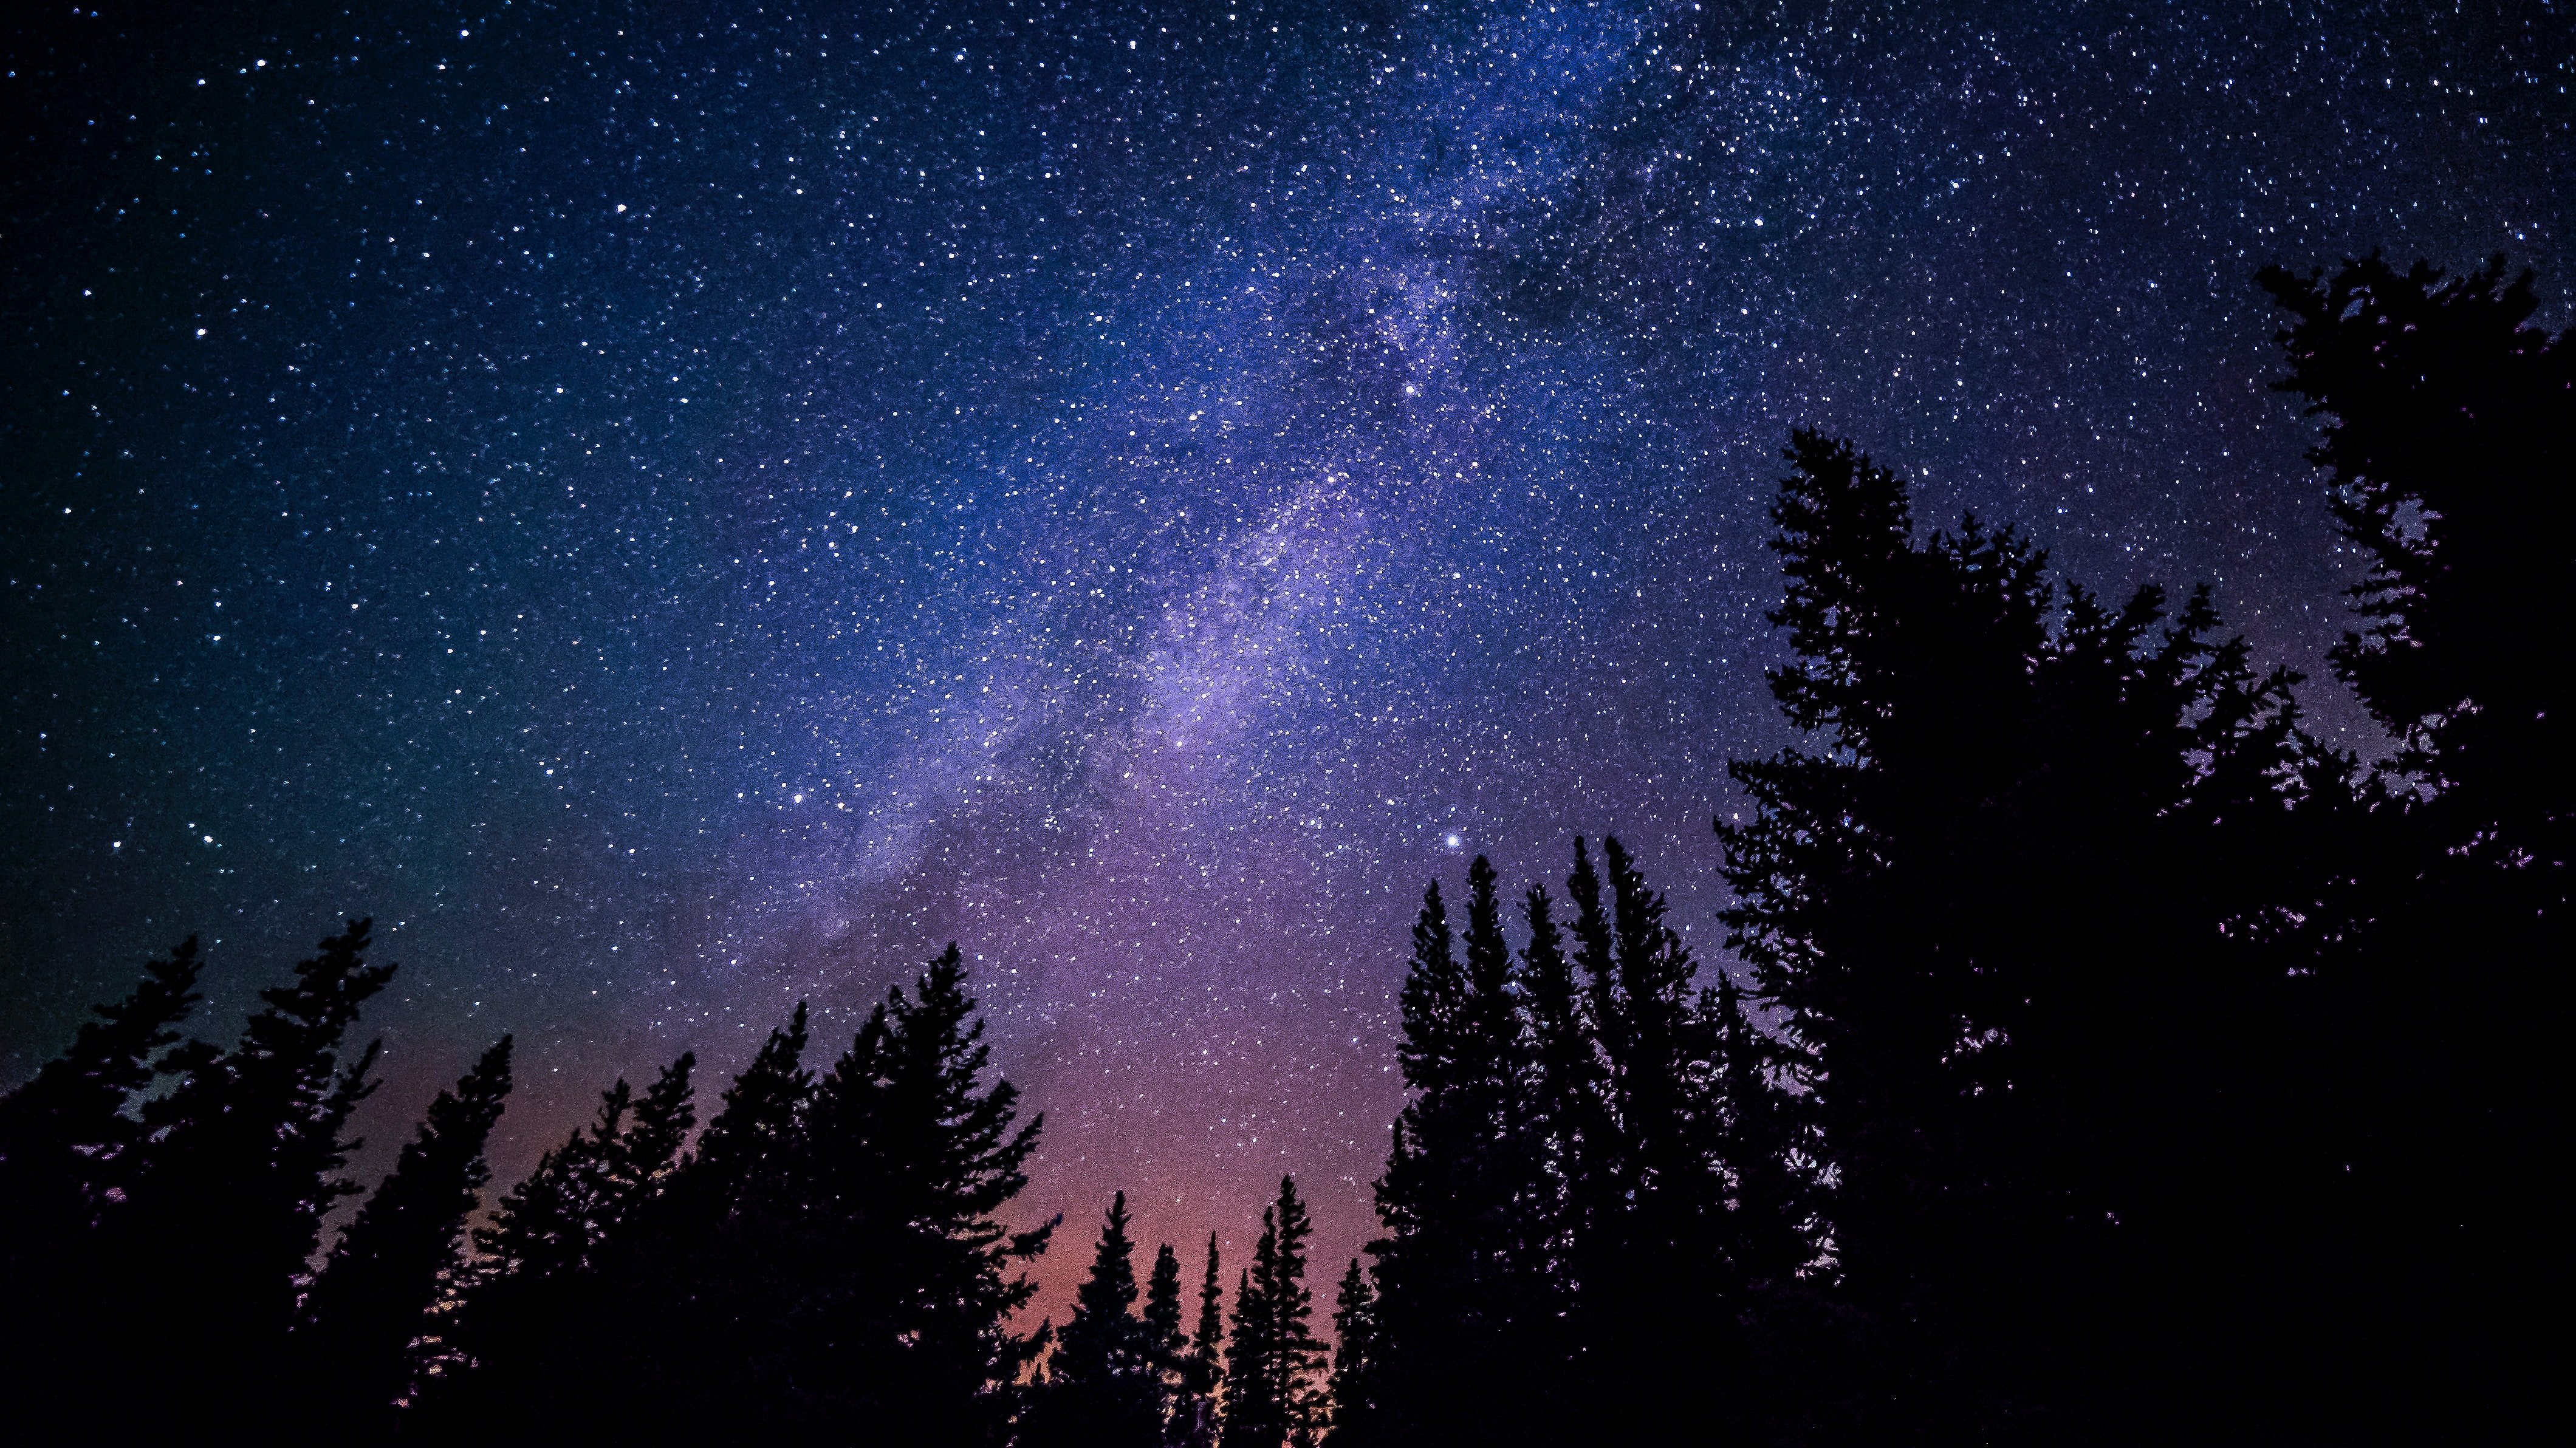
\includegraphics[width=1.4\paperwidth]{/home/melanie/Work/pictures/physics/stars.jpg}}

\begin{frame}[plain]

$\,$\\[8cm]

\textcolor{white}{Warum können wir die Sterne sehen, \\ aber nicht hören?} 

\end{frame}
}

 
%% Unterschied Schallwellen, elektromagnetische Wellen
\begin{frame}
\frametitle{Schallwellen brauchen ein Medium}

%%%%%%%%%%%%%%%%%%%%%%%%%%%%%%%%%%%%%
%% Schall-Licht-Tafel update: Medium
%%%%%%%%%%%%%%%%%%%%%%%%%%%%%%%%%%%%%
\begin{tabular}{|l|l|l|}
\hline
        & \color{theme}{\textbf{Schallwellen}}  & \color{theme}{\textbf{Elektromagnetische Wellen}}     \\
\hline
Ausbreitung       & \SI{330}{\meter\per\second} (Luft)  &  \(\sim\)\SI{300\,000\,000}{\meter\per\second} (Vakuum)   \\
\hline
Richtung        & longitudinal  & transversal   \\
\hline
Medium          & nötig (z.B. Luft)        & nicht nötig \\ 
&                       & (können sich im Vakuum ausbreiten)       \\
\hline
\end{tabular}
\end{frame}


%% %% Schallstärke

\begin{frame}
\frametitle{Schallstärke}

\[
\text{Schallstärke in Bel} = \lg \frac{\text{Schallstärkepegel}}{\text{Vergleichspegel}} 
\]

$\,$\\

Maßeinheit für den Schallstärkepegel und für den Vergleichspegel ist W/m$^2$ - fällt bei Division weg.  \\

Der Vergleichspegel ist festgelegt mit \(10^{-12}\,\frac{\text{W}}{m^2}\) \\

\pause

\[1\,\text{Dezibel} = 0.1\,\text{Bel}\]

\pause

Fragen:
\begin{itemize}
\item
Was ist die Schallstärke (in Bel) bei einem Schallstärkepegel von \(10^{-12}\,\frac{\text{W}}{m^2}\)?
\item
Was ist die Schallstärke (in Dezibel) bei einem Schallstärkepegel von \(10^{-12}\,\frac{\text{W}}{m^2}\)?
\item
Um wieviel ändert sich der Dezibel-Wert, wenn sich die Schallstärke verdoppelt?
\end{itemize}



\end{frame}



\begin{frame}
\frametitle{Schallstärke}

\begin{itemize}
\item
Was ist die Schallstärke (in Bel) bei einem Schallstärkepegel von \(10^{-12}\,\frac{W}{m^2}\)?

\end{itemize}


\[
\text{Schallstärke in Bel} = \lg \frac{\text{Schallstärkepegel}}{\text{Vergleichspegel}} 
\]

$\,$\\

Der Vergleichspegel ist festgelegt mit \(10^{-12}\,\frac{W}{m^2}\) \\


\[
\text{Schallstärke in Bel} = \lg \frac{10^{-12}\,\frac{\text{W}}{m^2}}{10^{-12}\,\frac{W}{m^2}}  = \lg 1 = 0\,\text{Bel}
\]




\end{frame}




\begin{frame}
\frametitle{Schallstärke}

\begin{itemize}
\item
Was ist die Schallstärke (in \emph{Dezibel}) bei einem Schallstärkepegel von \(10^{-12}\,\frac{W}{m^2}\)?

\end{itemize}

\[1\,\text{Dezibel} = 0.1\,\text{Bel}\]


\[
0.1 \times 0\,\text{Bel} = 0\,\text{Dezibel}
\]

\end{frame}


\begin{frame}
\frametitle{Schallstärke}


\begin{itemize}
\item
Um wieviel ändert sich der Dezibel-Wert, wenn sich die Schallstärke verdoppelt?
\end{itemize}

\[
D_2 - D_1 = 10\times \lg \frac{\text{Schallstärkepegel}_2}{\text{Vergleichspegel}} - 10\times \lg \frac{\text{Schallstärkepegel}_1}{\text{Vergleichspegel}} =
\]

\pause

\[
= 10 \times \left( \lg \frac{\text{Schallstärkepegel}_2}{\text{Vergleichspegel}} -  \lg \frac{\text{Schallstärkepegel}_1}{\text{Vergleichspegel}} \right)  =
\]

\pause


\[
= 10 \times \lg \frac{\frac{\text{Schallstärkepegel}_2}{\text{Vergleichspegel}}}{\frac{\text{Schallstärkepegel}_1}{\text{Vergleichspegel}}} =
\]

\pause


\[
= 10 \times \lg \frac{\text{Schallstärkepegel}_2}{\text{Schallstärkepegel}_1} =
\]

\pause


\[
= 10 \times \lg  \frac{2\times \text{Schallstärkepegel}_1}{\text{Schallstärkepegel}_1} = 10 \lg 2 = 3
\]


\end{frame}




%% Hörbares Spektrum 



\begin{frame}
\makebox[\linewidth]{\includegraphics[page=49,width=\textwidth]{Walter_Wellen.pdf}}
\end{frame}


%% Lautstärke

\begin{frame}
\frametitle{In Wirklichkeit ist es komplizierter}
\pause

Hörbarkeit hängt von der Frequenz \emph{und} der Schallstärke ab

\begin{center}
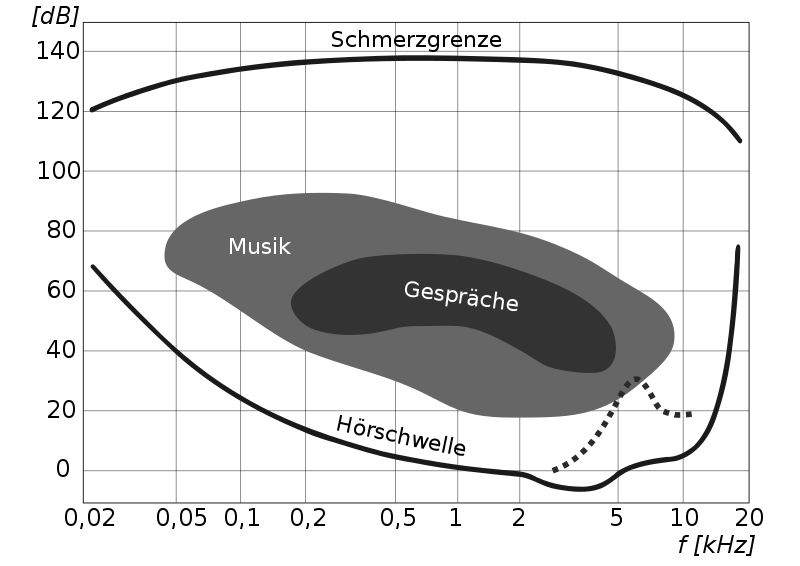
\includegraphics[width=0.8\textwidth]{/home/melanie/Work/pictures/medicine/Hoerflaeche.png}
\end{center}

\end{frame}

%% Phon

\begin{frame}
\makebox[\linewidth]{\includegraphics[page=52,width=\textwidth]{Walter_Wellen.pdf}}
\end{frame}

\begin{frame}
\makebox[\linewidth]{\includegraphics[page=53,width=\textwidth]{Walter_Wellen.pdf}}
\end{frame}

\begin{frame}
\makebox[\linewidth]{\includegraphics[page=54,width=\textwidth]{Walter_Wellen.pdf}}
\end{frame}


%% Ultraschall

\begin{frame}
\frametitle{Anwendung von Schallwellen: Ultraschall-Diagnostik}

Schall wird von unterschiedlichen Geweben unterschiedlich reflektiert. Ultraschall ist nicht gefährlich und nicht schmerzhaft.

\begin{center}
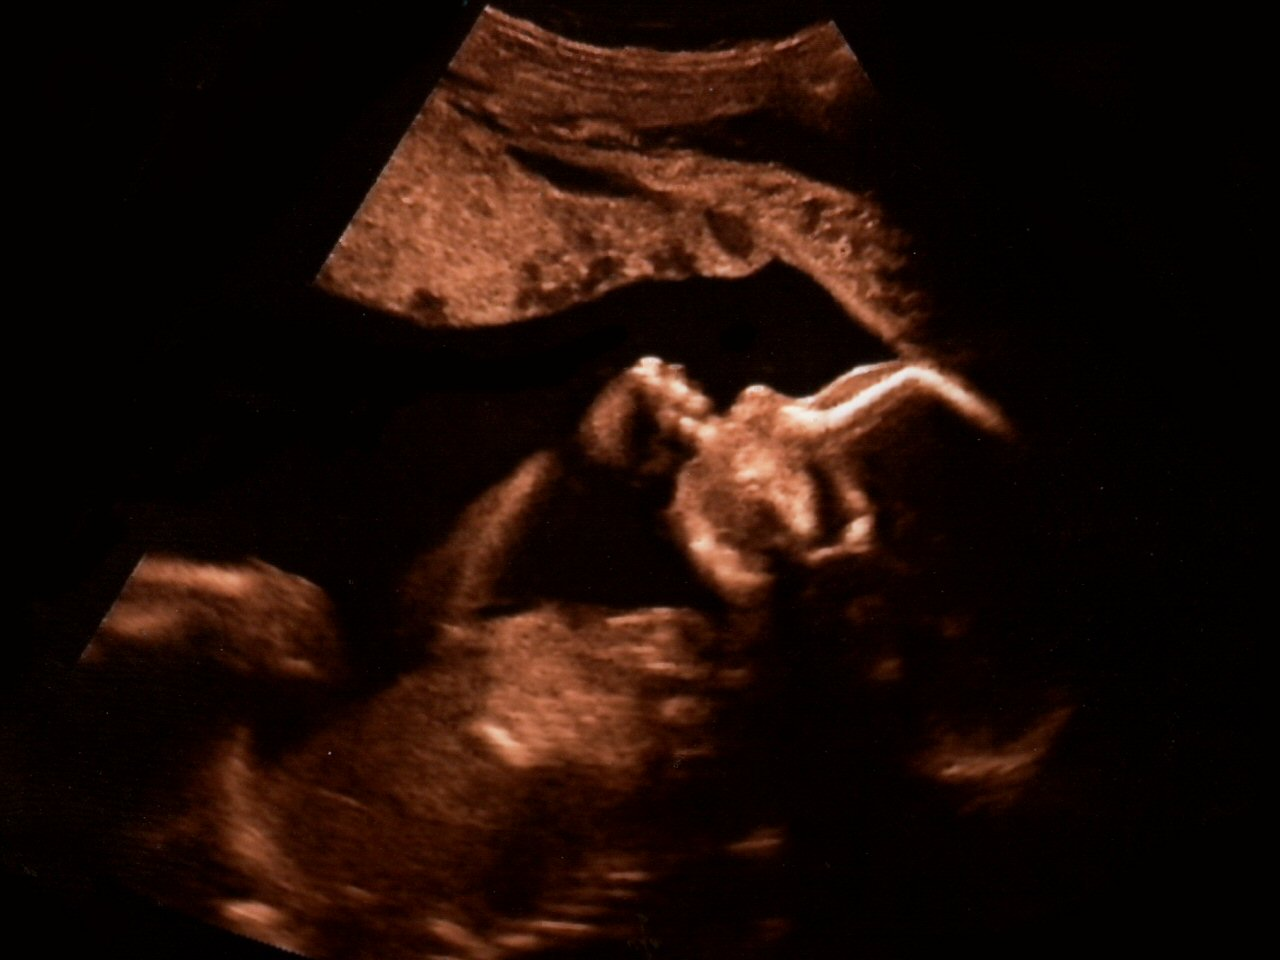
\includegraphics[width=0.6\textwidth]{/home/melanie/Work/pictures/medicine/embryo.jpg}
\end{center}



\end{frame}


%% Übung: Beispiele von Konzepten, die wir schon kennen
\begin{frame}

\frametitle{Schallwellen als Wellen}

Folgende Phänomene haben wir bereits als allgemeine Wellen-Phänomene kennen gelernt. Treffen sie auch auf Schall-Phänomene zu? Fällt Ihnen ein Beispiel ein?


\begin{itemize}
\item
 Resonanz
\item
Resonanzkatastrophe
\item
 Schwebung
\item
 Doppler Effekt
\item
Fourier-Analyse
\end{itemize}

\end{frame}

\begin{frame}
\frametitle{Schallwellen als Wellen - Resonanz}


\begin{center}
\includegraphics<1>[width=\textwidth]{/home/melanie/Work/pictures/physics/piano_experiment_1.png}
\includegraphics<2>[width=\textwidth]{/home/melanie/Work/pictures/physics/piano_experiment_2.png}
\includegraphics<3>[width=\textwidth]{/home/melanie/Work/pictures/physics/piano_experiment_3.png}
\includegraphics<4>[width=\textwidth]{/home/melanie/Work/pictures/physics/piano_experiment_4.png}

\end{center}

\end{frame}



\begin{frame}
\frametitle{Schallwellen als Wellen - Resonanzkatastrophe}

\begin{center}
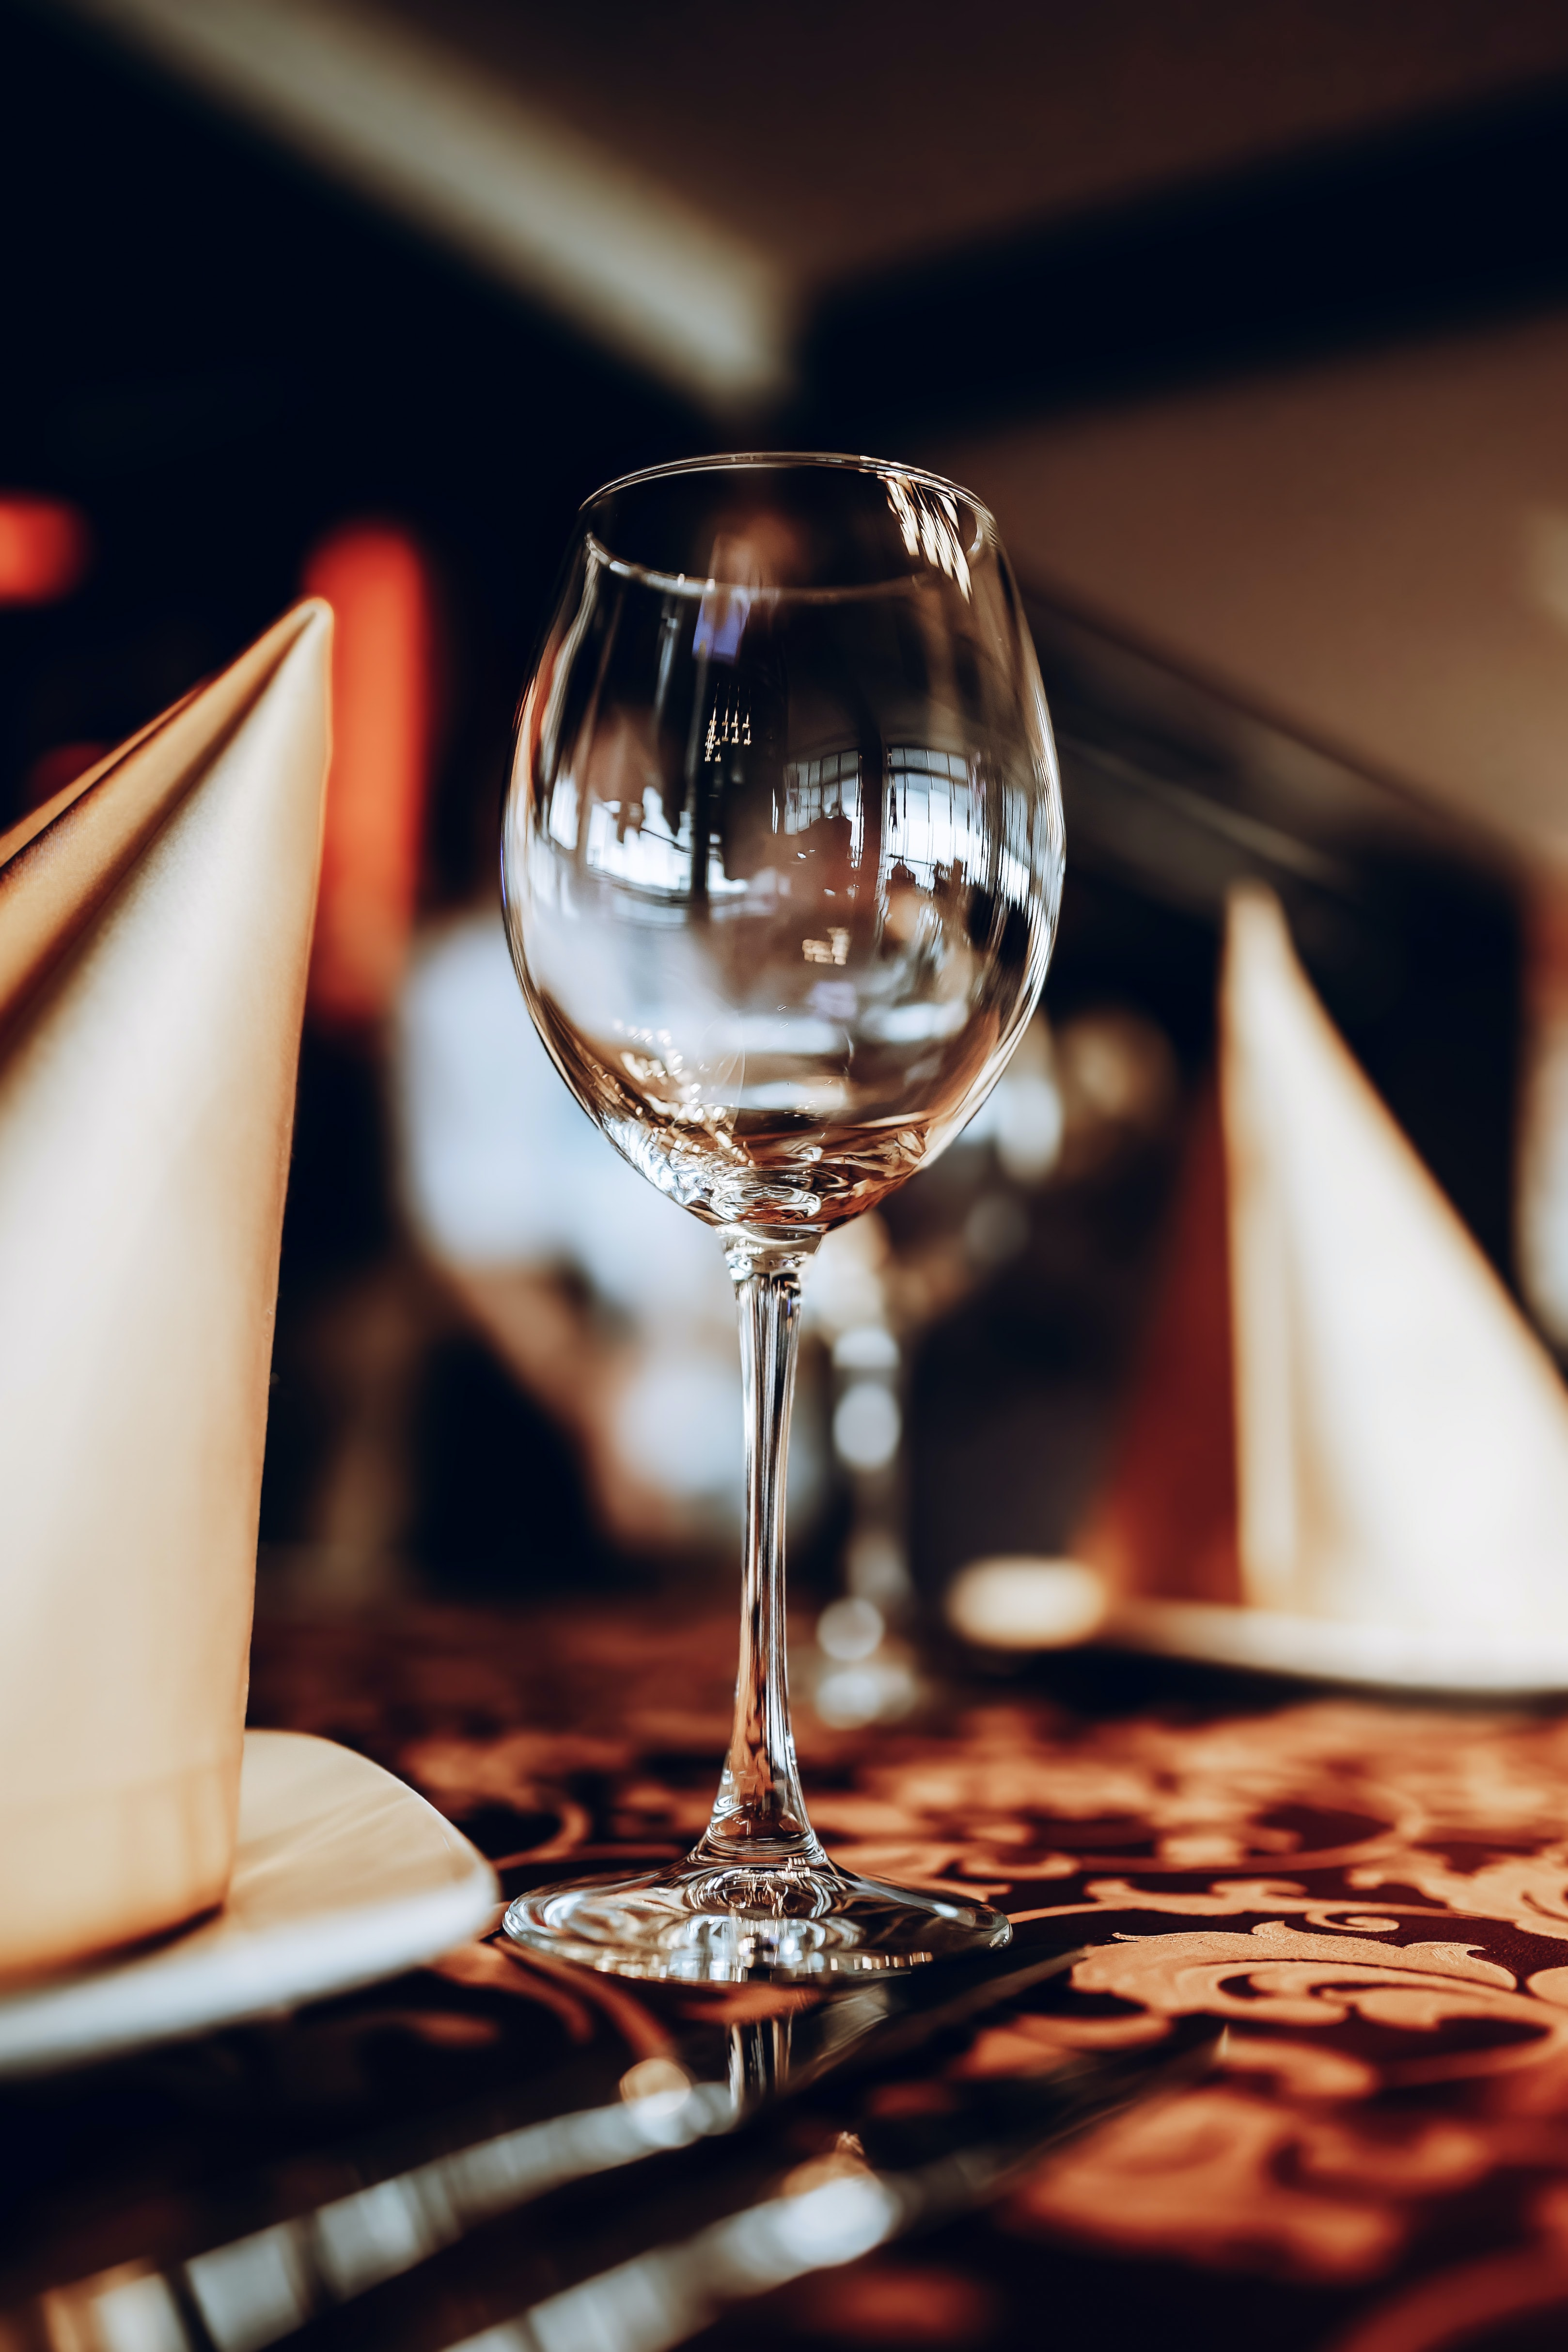
\includegraphics[width=0.4\textwidth]{/home/melanie/Work/pictures/physics/wine_glass.jpg}
\end{center}


\end{frame}


\begin{frame}
\frametitle{Schallwellen als Wellen - Schwebung}

\begin{center}
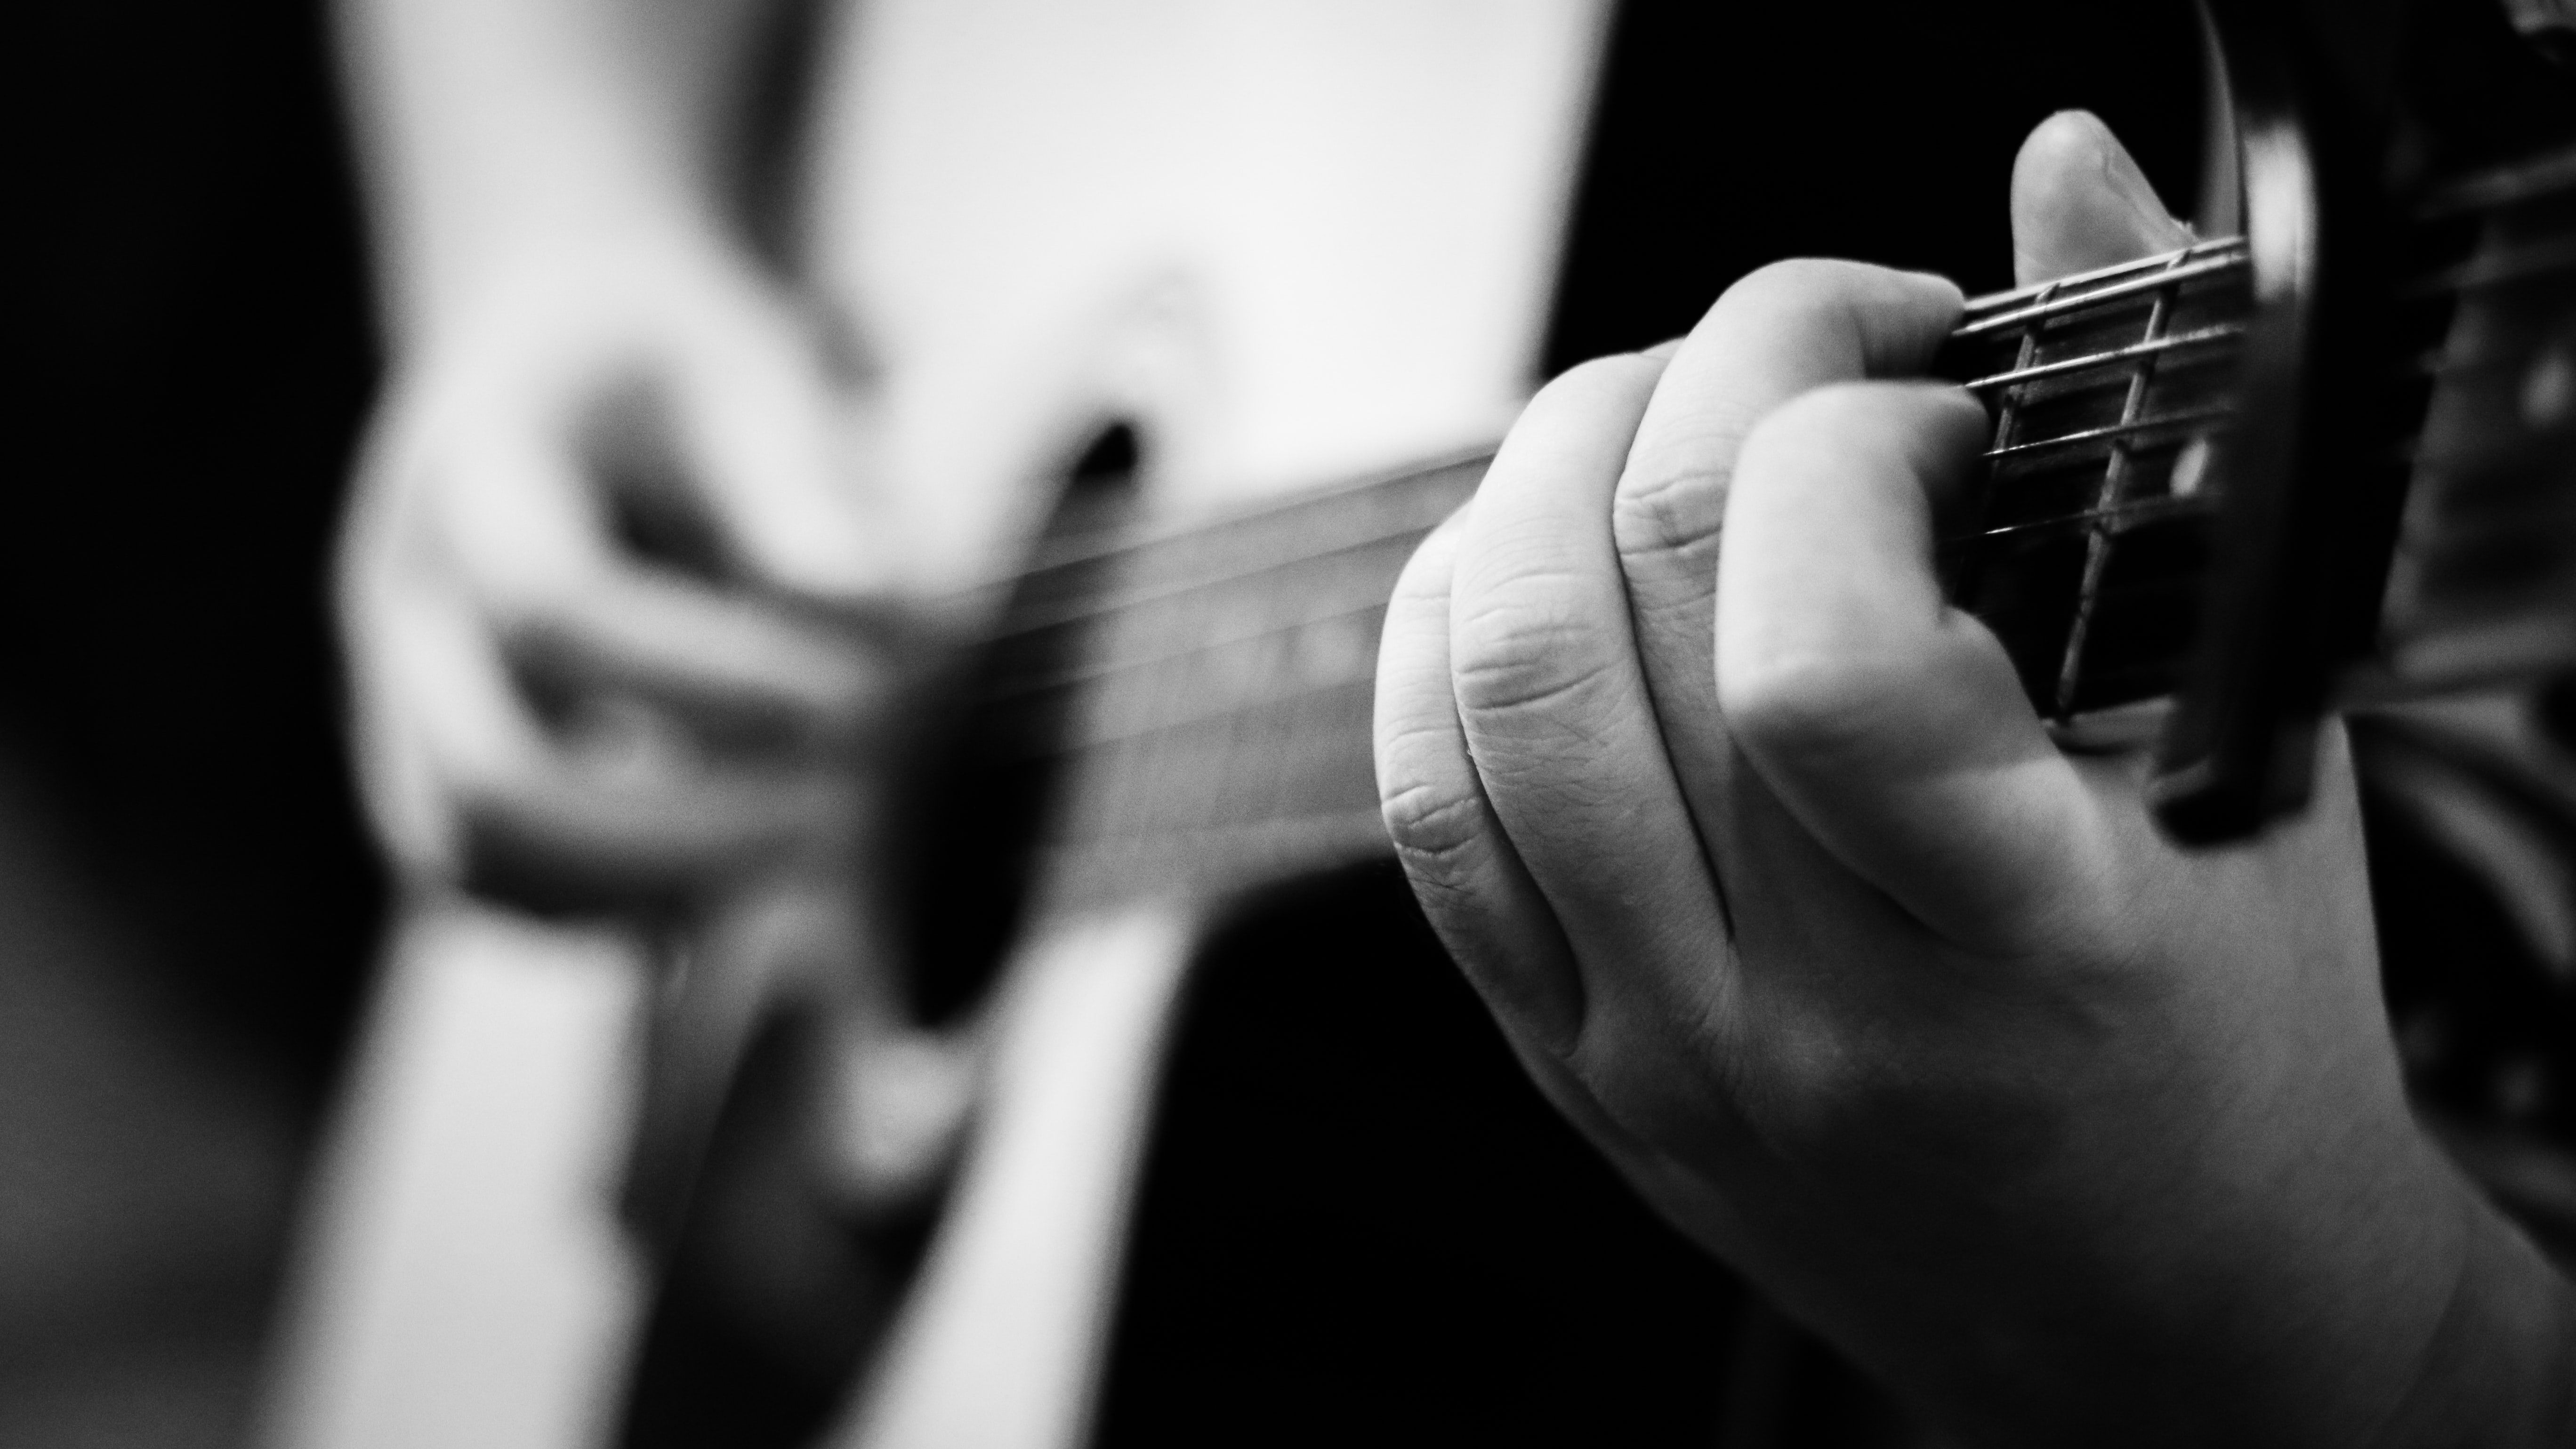
\includegraphics[width=\textwidth]{/home/melanie/Work/pictures/physics/guitar.jpg}
\end{center}


\end{frame}


\begin{frame}
\frametitle{Schallwellen als Wellen - Doppler Effekt}

\begin{center}
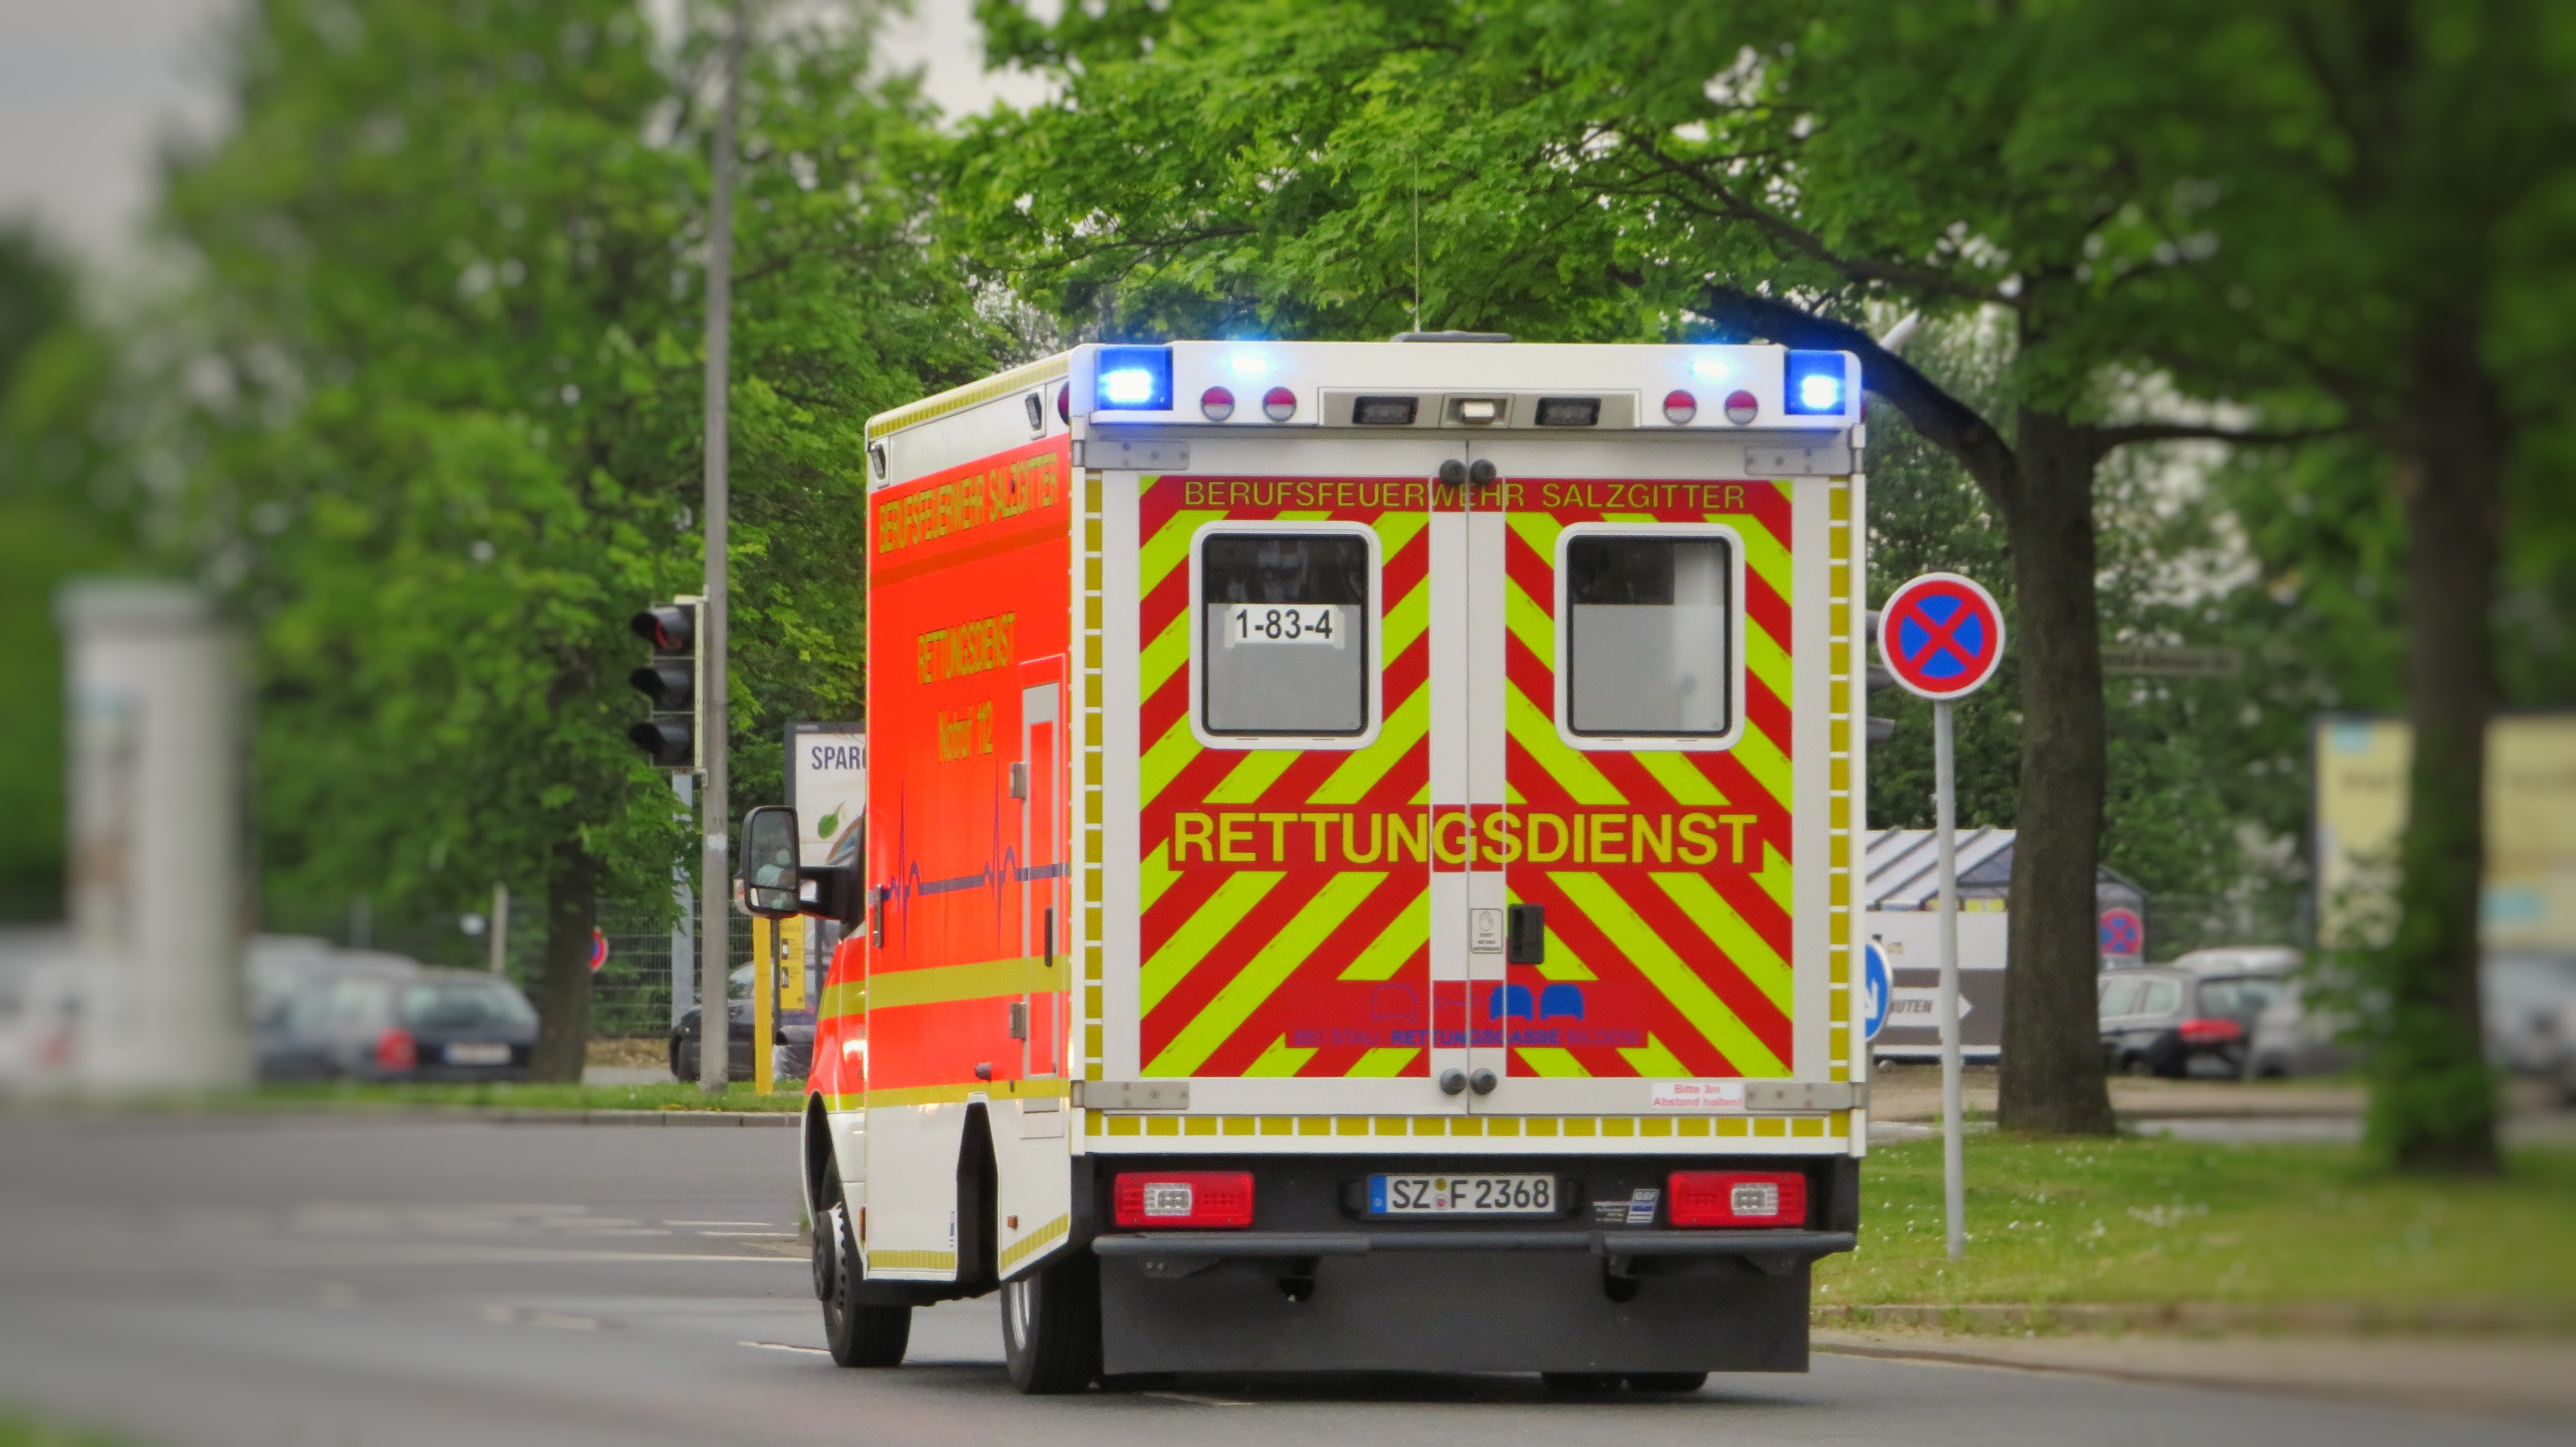
\includegraphics[width=\textwidth]{/home/melanie/Work/pictures/physics/krankenwagen.jpg}
\end{center}


\end{frame}



%% Hören: Mechanismus + Tinnitus

\begin{frame}
\frametitle{Mechanismus des Hörens}


\begin{center}
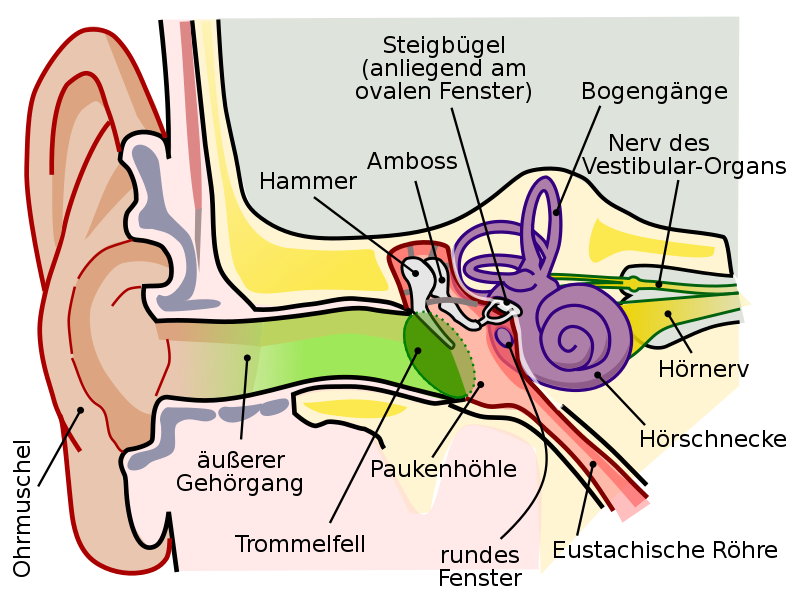
\includegraphics[width=0.8\textwidth]{/home/melanie/Work/pictures/medicine/Anatomy_of_the_Human_Ear.png}
\end{center}



\end{frame}

\begin{frame}
 \frametitle{Mechanismus des Hörens}

\begin{columns}[c]


\begin{column}{4cm}
\begin{center}
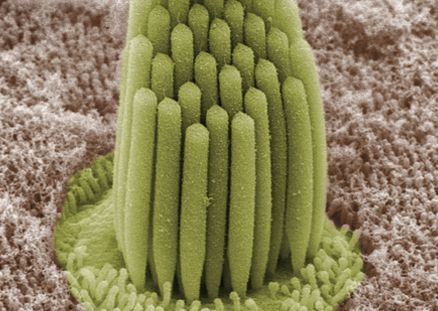
\includegraphics[width=\textwidth]{/home/melanie/Work/pictures/medicine/Stereocilia.jpg}
\end{center}
\end{column}

\pause

\begin{column}{7cm}
Schallwellen werden von Hammer, Amboss und Steigbügel verstärkt. In der Hörschnecke befindet sich Flüssigkeit, die durch die Schallwellen in Schwingung versetzt wird. Entlang der Hörschnecke sitzen Haarzellen, deren Zilien mit durch die Wellen in der Flüssigkeit mechanisch verformt wreden. Dadurch werden die Haarzellen aktiviert, und das Signal weiter ins Gehirn geleitet. Dabei sind verschiedene Haarzellen für verschiedene Frequenzen zuständig.   \\
\pause
\textcolor{theme}{\(\rightarrow\) In der Hörschnecke passiert eine Fourier-Analyse!}
\end{column}

\end{columns}

\end{frame}





%%%%%%%%%%%%%%%%%%%%%%%%%%%%%%%%%%%
%% Elektromagnetische Wellen
%%%%%%%%%%%%%%%%%%%%%%%%%%%%%%%%%%%


\section{Elektromagnetische Wellen}

%% Was sind elektromagnetische Wellen?
\begin{frame}
\frametitle{Was sind elektromagnetische Wellen?}

 Elektromagnetische Wellen sind Wellen aus gekoppelten magnetischen und elektrischen Feldern

\begin{center}
\includegraphics<1>[width=0.6\textwidth]{/home/melanie/Work/pictures/physics/elektromagnetische_wellen_entstehung_1.png}
\includegraphics<2>[width=0.6\textwidth]{/home/melanie/Work/pictures/physics/elektromagnetische_wellen_entstehung_2.png}
\includegraphics<3>[width=0.6\textwidth]{/home/melanie/Work/pictures/physics/elektromagnetische_wellen_entstehung_3.png}
\end{center}


\end{frame}


\begin{frame}
\frametitle{Was sind elektromagnetische Wellen?}

\centering
\animategraphics[loop, width=\textwidth]{5}{/home/melanie/Work/pictures/physics/EMW}{1}{31}


\end{frame}

\begin{frame}
\frametitle{Ok, aber was ist dieser ``Dipol''?}


\begin{columns}[c]
\begin{column}{5cm}
Elektromagnetische Wellen können auf unterschiedliche Arten entstehen. Z.B.:\\
\begin{itemize}
\item
Radiowellen: Antenne 
\item
Röntgenstrahlung: Beschleunigung geladener Teilchen 
\item
Fluoreszenz: Molekulare und atomare Prozesse
\end{itemize}
\end{column}


\begin{column}{5cm}
\begin{center}
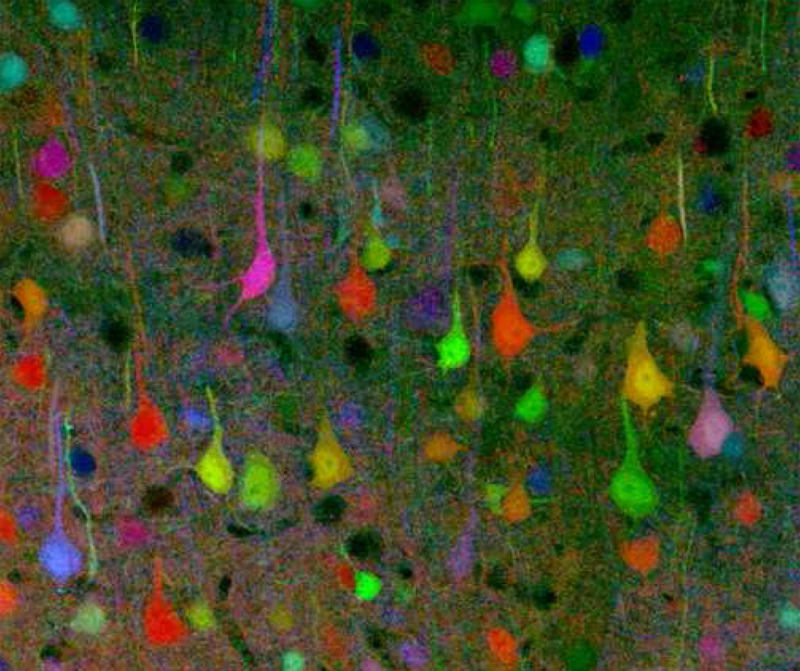
\includegraphics[width=\textwidth]{/home/melanie/Work/pictures/brain/Brainbow.jpg}
\end{center}


\end{column}

\end{columns}

\end{frame}


%% Was unterscheidet elektromagnetische Wellen von Schallwellen?
\begin{frame}
\frametitle{Was unterscheidet elektromagnetische Wellen von Schallwellen?}

\pause

\begin{tabular}{|l|l|l|}
\hline
        & \color{theme}{\textbf{Schallwellen}}  & \color{theme}{\textbf{Elektromagnetische Wellen}}     \\
\hline
Ausbreitung       & \SI{330}{\meter\per\second} (Luft)  &  \(\sim\)\SI{300\,000\,000}{\meter\per\second} (Vakuum)   \\
\hline
Richtung        & longitudinal  & transversal   \\
\hline
Medium          & nötig (z.B. Luft)        & nicht nötig \\ 
&                       & (können sich im Vakuum ausbreiten)       \\
\hline
\end{tabular}


\end{frame}


%% Elektromagnetische Wellen: Spektrum, Frequenzen
\begin{frame}
\frametitle{Elektromagnetisches Spektrum}

\begin{center}
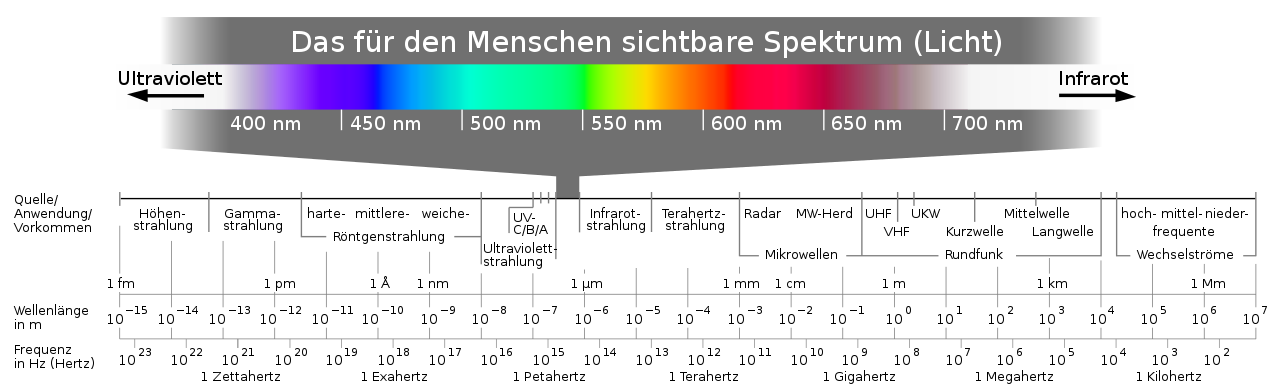
\includegraphics[width=\textwidth]{/home/melanie/Work/pictures/physics/Electromagnetic_spectrum.png}
\end{center}

\end{frame}


%% Beispiel: Seerosen

%% Sneak preview: Optik

\begin{frame}
\frametitle{Mehr zu elektromagnestichen Wellen \dots}


\begin{center}
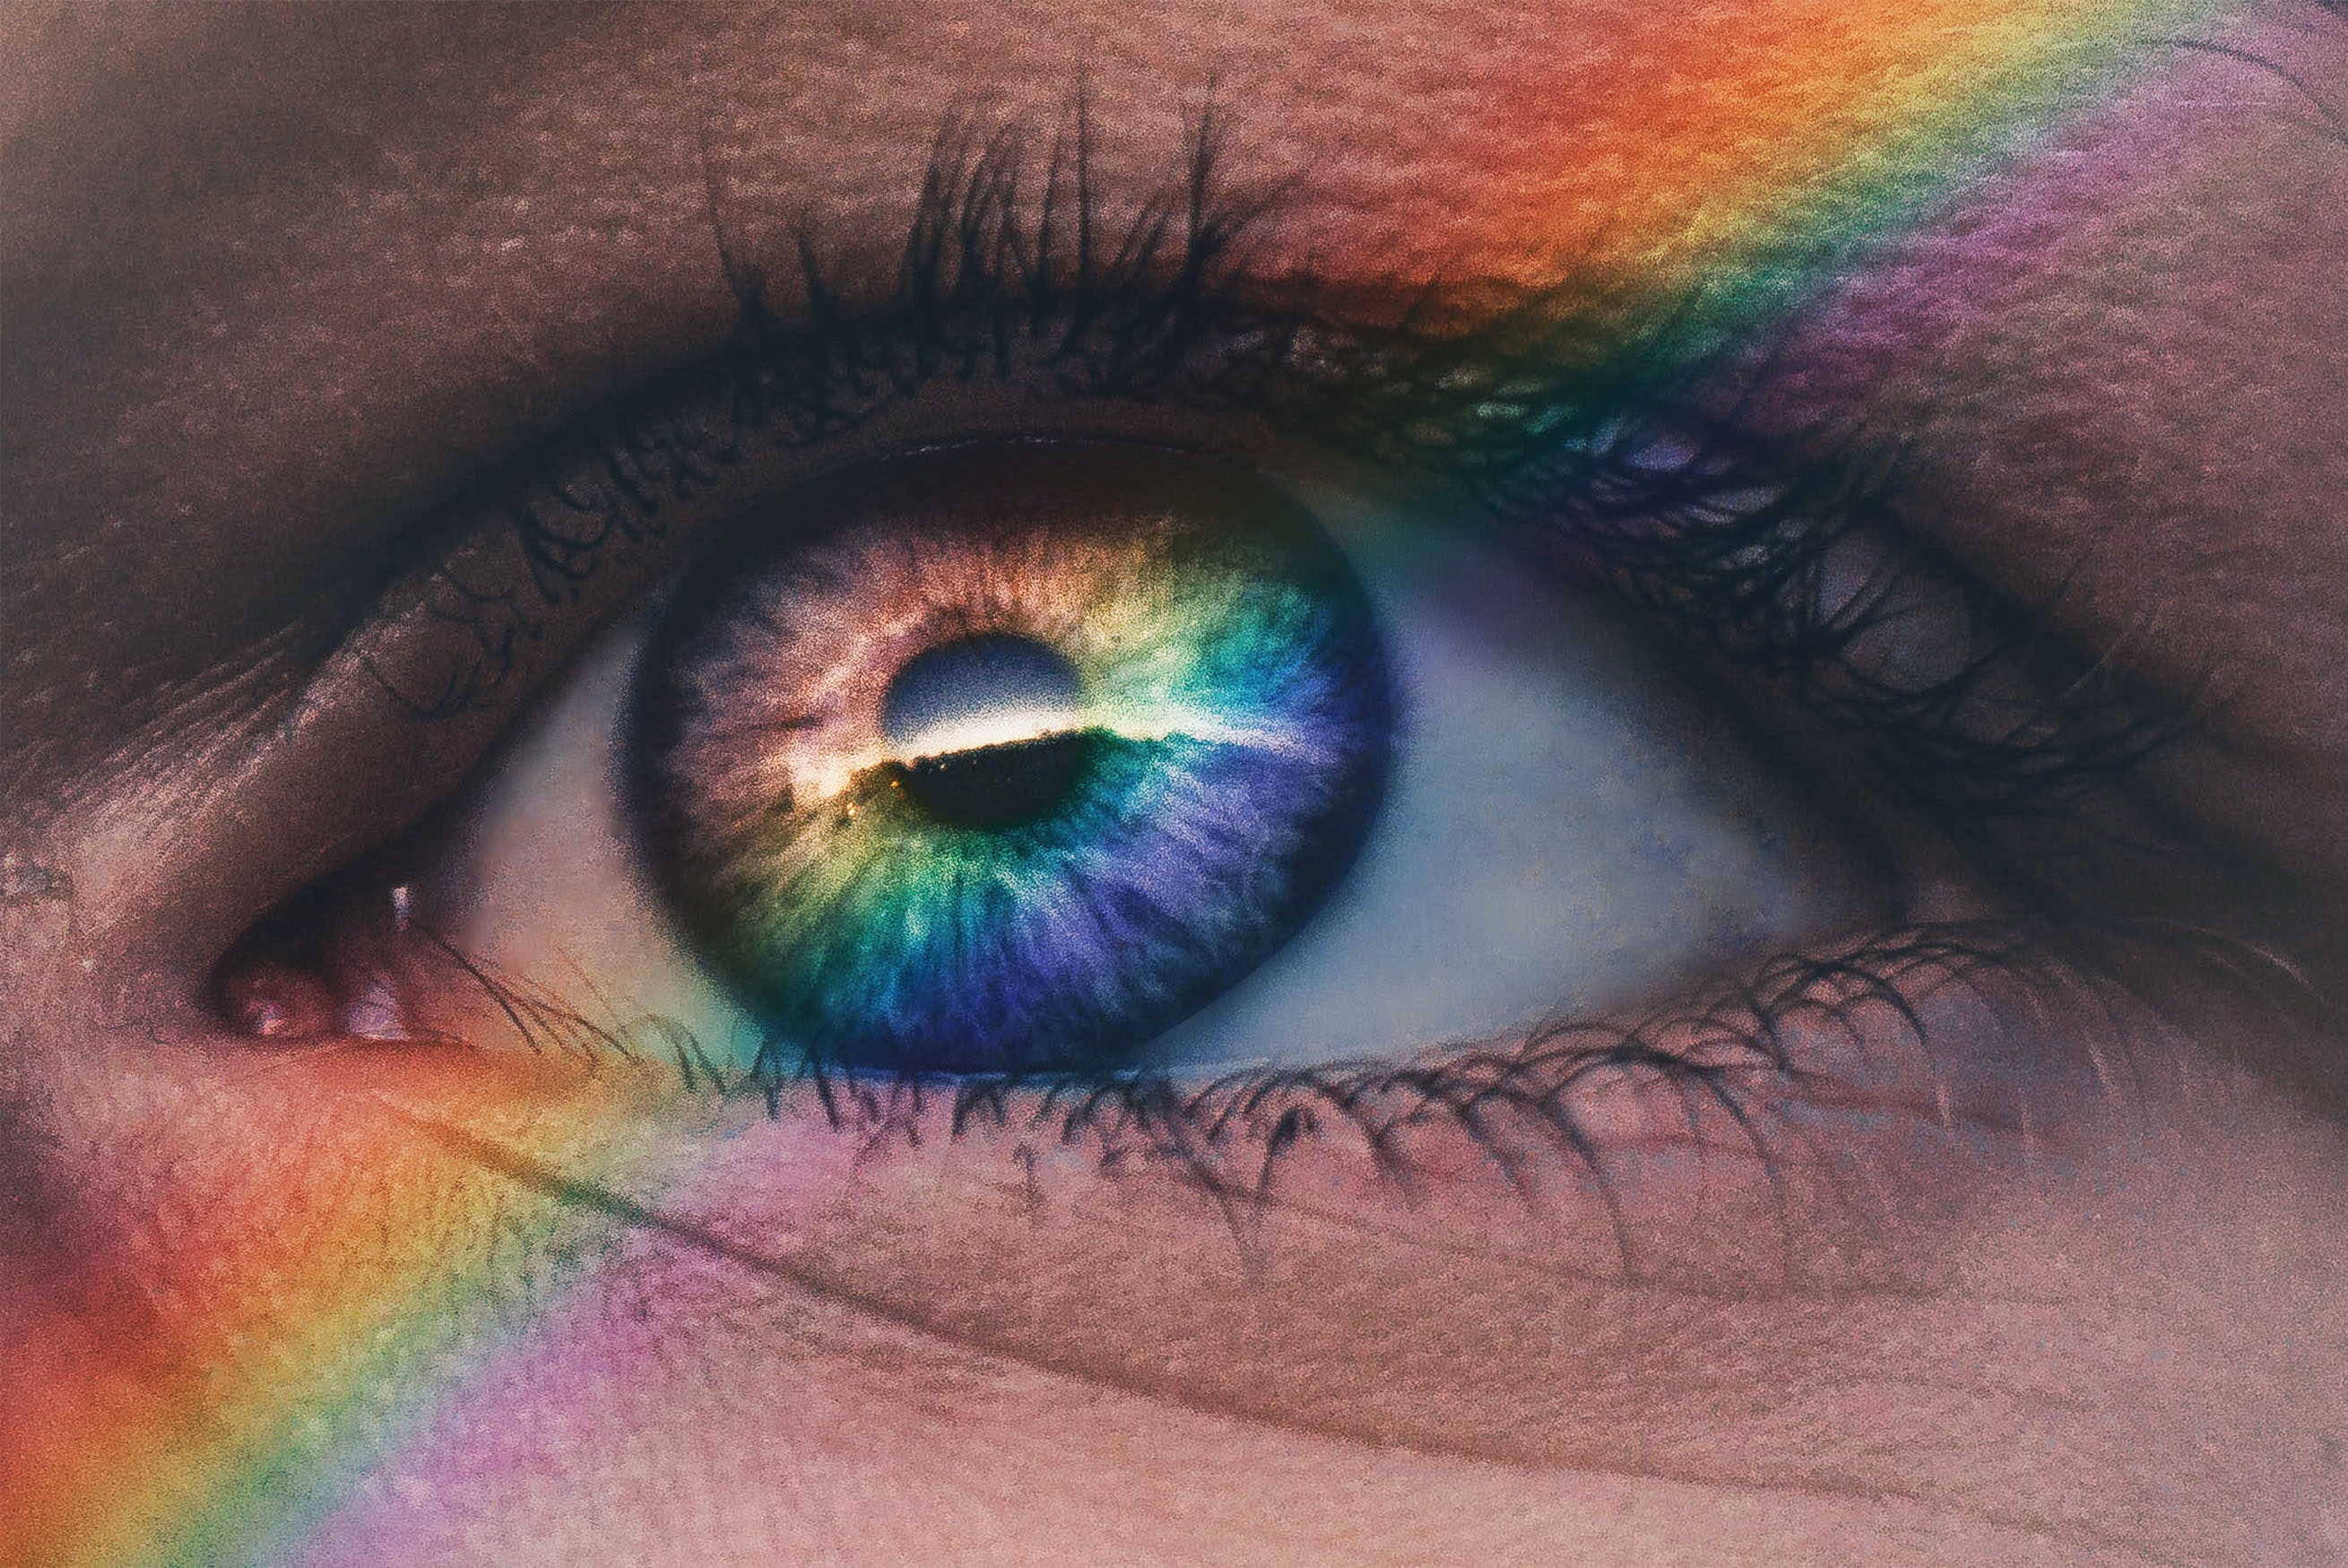
\includegraphics[width=0.8\textwidth]{/home/melanie/Work/pictures/physics/rainbow_eye.jpg}
\end{center}

\dots in der Vorlesung über Optik!


\end{frame}





%% Review
\begin{frame}

\frametitle{Jetzt* sollten Sie:}

\begin{block}{Wissen:}
\begin{itemize}
%%%%%
\item
Schwingungen und Wellen definieren
\item
Charakteristika von Schwingungen und Wellen benennen 
\item
Arten von Schwingungen und Wellen unterscheiden
\item
Erzwungene Schwingungen definieren und erklären
\item
Phänomene bei der Überlagerung von Wellen erklären
\item
Den Doppler-Effekt erklären
\item
Beispiele für den Doppler-Effekt geben
\item
Eigenschaften von Schallwellen benennen
\item
Eigenschaften elektromagnetischer Wellen benennen
\item
Unterschiede und Gemeinsamkeiten zwischen elektromagnetischen Wellen und Schallwellen angeben
\item
Das Konzept der Fourieranalyse erklären und Anwendungen nennen
\end{itemize} 

\end{block}

\end{frame}



\begin{frame}

\frametitle{Jetzt* sollten Sie:}

\begin{block}{Können:}
\begin{itemize}
\item
Charakteristika von Schwingungen und Wellen berechnen
\item
Graphische Darstellungen von Schwingungen und Wellen interpretieren
\item
Änderungen der Schallstärke berechnen
\item
Mit Klavieren experimentieren (und auch sonst) 
\end{itemize}
\end{block}

\begin{block}{Fühlen:}

\begin{itemize}
\item
Keine Angst vor Fouriertransformationen haben
\item
Schwingungen und Wellen im Alltag sehen 


\end{itemize}

\end{block}


\end{frame}

%% Feedbackhinweisblock

\begin{frame}
\frametitle{Danke für Ihr Feedback!}

\begin{columns}[c]

\begin{column}{6cm}
\begin{center}

\includegraphics[width=\textwidth]{/home/melanie/Work/pictures/metaphore/smilie_balloons.jpg}
\end{center}

\end{column}

\begin{column}{4cm}


\begin{center}

\includegraphics[width=\textwidth]{feedback_QR.png}
\end{center}
\end{column}


\end{columns}

\end{frame}





%% Bildnachweis
\begin{frame}
\frametitle{Bildnachweis}
\begin{tiny}
Diese Vorlesung verwendet teilweise Materialien (Folien und Bilder) einer früheren Vorlesung von Prof. Wim Walter.  Wo nicht anders nachgewiesen, sind auch Bilder aus dieser Vorlesung. 
\end{tiny}

\vfill

\begin{tiny}
 
\begin{itemize}

\item
Aufeinander treffende Wasserwellen. Photo by \href{https://unsplash.com/@dreamsoftheoceans?utm_source=unsplash&utm_medium=referral&utm_content=creditCopyText}{Linus Nylund} on \href{https://unsplash.com/s/photos/water-ripples?utm_source=unsplash&utm_medium=referral&utm_content=creditCopyText}{Unsplash}
  
\item
Auge mit Regenbogen. Photo by \href{https://unsplash.com/@mango_quan?utm_source=unsplash&utm_medium=referral&utm_content=creditCopyText}{Harry Quan} on \href{https://unsplash.com/s/photos/prism?utm_source=unsplash&utm_medium=referral&utm_content=creditCopyText}{Unsplash}
  
\item
Ausbreitung elektromagnetischer Wellen. Von And1mu - Eigenes Werk, CC BY-SA 4.0, \url{https://commons.wikimedia.org/w/index.php?curid=49759107}

\item
Brainbow. By Stephen J Smith - \url{https://www.ncbi.nlm.nih.gov/pmc/articles/PMC2693015/}, CC BY 3.0, \url{https://commons.wikimedia.org/w/index.php?curid=25703414}

\item
Doppler-Sonogramm.Von schomynv 06:41, 19. Dez. 2008 (CET) - schomynv 06:41, 19. Dez. 2008 (CET), CC BY-SA 3.0, \url{https://de.wikipedia.org/w/index.php?curid=4058483}

\item
Eigenschaften von Schwingungen. Meine eigene Arbeit, CC BY-SA 4.0 2022.

\item
Elektromagnetisches Spektrum. Horst Frank / Phrood / Anony, CC BY-SA 3.0 \url{http://creativecommons.org/licenses/by-sa/3.0/}, via Wikimedia Commons

\item
Entstehung elektromagnetischer Wellen. Meine eigene Arbeit, CC BY-SA 4.0, 2022.

\item
Evelyn Glennie. Photo, may 30, 2004- photo: nomo/michael hoefner \url{http://www.zwo5.de} CC-BY-SA 2.5 via Wikimedia Commons.

\item
Fortbewegung des Regenwurms. lilaandben. Der Regenwurm, 2022. \url{https://lilaundben.mediastart.de/de/gartenzwerg/der-regenwurm}

\item
Gewitter. Photo by \href{https://unsplash.com/@alienaperture?utm_source=unsplash&utm_medium=referral&utm_content=creditCopyText}{Michael D} on \href{https://unsplash.com/s/photos/thunderstorm?utm_source=unsplash&utm_medium=referral&utm_content=creditCopyText}{Unsplash}

\item
Gitarre. Photo by \href{https://unsplash.com/@wooozxh?utm_source=unsplash&utm_medium=referral&utm_content=creditCopyText}{Zhang Xue Huan} on \href{https://unsplash.com/s/photos/tuning-guitar?utm_source=unsplash&utm_medium=referral&utm_content=creditCopyText}{Unsplash}
  
  
\item
Haarzelle mit Zilien (im Frosch). By Bechara Kachar - \url{http://irp.nih.gov/our-research/research-in-action/high-fidelity-stereocilia/slideshow}, Public Domain, \url{https://commons.wikimedia.org/w/index.php?curid=24468731}

\item
Hörfläche. Von Hoerflaeche.svg: TehdogLukeTriton - Based on a SVG Drawing Datei:Hoerflaeche.svg.SVG drawing: Eigenes Werk (Originaltext: retraced as svg, copyright info taken from original), Gemeinfrei, \url{https://commons.wikimedia.org/w/index.php?curid=114265551}

\end{itemize}
\end{tiny}
\end{frame}

\begin{frame}
\frametitle{Bildnachweis}

\begin{tiny}

\begin{itemize}


\item
Kind auf einer Schaukel. Photo by \href{https://unsplash.com/@mylestan?utm_source=unsplash&utm_medium=referral&utm_content=creditCopyText}{Myles Tan} on \href{https://unsplash.com/s/photos/swing?utm_source=unsplash&utm_medium=referral&utm_content=creditCopyText }{Unsplash}
  
\item
Kind auf einer Schaukel als Fadenpendel. Meine eigene Arbeit, CC BY-SA 4.0, 2022. 

\item
Klavierexperiment. Eigene Arbeit, CC BY-SA 4.0, 2022.

\item
Krankenwagen. Photo by \href{https://unsplash.com/@augustinfoto?utm_source=unsplash&utm_medium=referral&utm_content=creditCopyText}{Jonas Augustin} on \href{https://unsplash.com/s/photos/krankenwagen?utm_source=unsplash&utm_medium=referral&utm_content=creditCopyText}{Unsplash}
  

%% all lectures
\item
Logo der MSB. MSB Medical School Berlin, Public Domain, via Wikimedia Commons
%%%%%%%%%%%%


%% all lectures
\item
Luftballons mit frohen und traurigen Smilies. Photo by \href{https://unsplash.com/@artbyhybrid?utm_source=unsplash&utm_medium=referral&utm_content=creditCopyText}{Hybrid} on \href{https://unsplash.com/s/photos/feedback?utm_source=unsplash&utm_medium=referral&utm_content=creditCopyText}{Unsplash}
%%%%%%%%%%%

\item
Mobiltelefon mit Kopfhörern. Photo by \href{https://unsplash.com/@firmbee?utm_source=unsplash&utm_medium=referral&utm_content=creditCopyText}{Firmbee.com} on \href{https://unsplash.com/s/photos/mp3?utm_source=unsplash&utm_medium=referral&utm_content=creditCopyText}{Unsplash}
  

\item
Noise cancelling Kopfhörer. Photo by \href{https://unsplash.com/@sjcbrn?utm_source=unsplash&utm_medium=referral&utm_content=creditCopyText}{SJ .} on \href{https://unsplash.com/s/photos/noise-cancelling-headphones?utm_source=unsplash&utm_medium=referral&utm_content=creditCopyText}{Unsplash}  

\item
Ohr. Von Lars Chittka; Axel Brockmann - Perception Space—The Final Frontier, A PLoS Biology Vol. 3, No. 4, e137 doi:10.1371/journal.pbio.0030137 (Fig. 1A/Large version), vectorised by Inductiveload, CC BY 2.5, \url{https://commons.wikimedia.org/w/index.php?curid=5957984}

\item
Sinuswellen. Es wird LucasVB als Autor angenommen (basierend auf den Rechteinhaber-Angaben). Gemeinfrei, \url{https://commons.wikimedia.org/w/index.php?curid=1536518}.  

\item
Sternenhimmel. Photo by \href{https://unsplash.com/@ryan_hutton_?utm_source=unsplash&utm_medium=referral&utm_content=creditCopyText}{Ryan Hutton} on \href{https://unsplash.com/s/photos/stars?utm_source=unsplash&utm_medium=referral&utm_content=creditCopyText}{Unsplash}

\item
Tacoma Narrows Bridge. UW Digital Collections, No restrictions, via Wikimedia Commons.

\item
Ultraschallbild eines Embryos. Von Havelbaude, CC BY-SA 3.0, \url{https://commons.wikimedia.org/w/index.php?curid=13378650}

\item
Umrechnung zwischen Zeit- und Frequenzbereich bei der Fourier-Analyse. Von Lucas V. Barbosa - Eigenes Werk, Gemeinfrei, \url{https://commons.wikimedia.org/w/index.php?curid=24830373}

\item
Weinglas. Photo by \href{https://unsplash.com/@tengyart?utm_source=unsplash&utm_medium=referral&utm_content=creditCopyText}{Tengyart} on \href{https://unsplash.com/s/photos/empty-wine-glass?utm_source=unsplash&utm_medium=referral&utm_content=creditCopyText}{Unsplash}
  

\item
Wellen im Meer. Photo by \href{https://unsplash.com/@lauraashtonashley?utm_source=unsplash&utm_medium=referral&utm_content=creditCopyText}{Laura Barry} on \href{https://unsplash.com/s/photos/waves?utm_source=unsplash&utm_medium=referral&utm_content=creditCopyText}{Unsplash}
  

\end{itemize}
\end{tiny}
\end{frame}


\end{document}
